\documentclass[a4paper,12pt, openany]{extbook}
% %%%%%%%%%%%%%%%%%%%%%%%%%%%%%%%%%%%%%%%%%
% % LaTeX Template
% % Version 1.0
% %
% % This template originates from:
% % http://www.LaTeXTemplates.com
% %
% % Authors:
% % Rocco Lo Russo (https://github.com/roccolr)
% %%%%%%%%%%%%%%%%%%%%%%%%%%%%%%%%%%%%%%%%%


%----------------------------------------------------------------------------------------
%	PACKAGES AND OTHER DOCUMENT CONFIGURATIONS
%----------------------------------------------------------------------------------------
\usepackage{subcaption} % Subfigures
\usepackage{float}
\usepackage{booktabs, colortbl} % aggiungi vicino agli altri \usepackage, se non già presenti

\usepackage{amsmath,amsfonts,stmaryrd,amssymb, mathtools} % Math packages
\everymath{\displaystyle\Large}

% --- NUMERAZIONE ---
\numberwithin{chapter}{part}
\renewcommand{\thechapter}{\arabic{chapter}}

\usepackage[italian]{babel}   % opzionale: titoli in italiano ("Indice", "Bibliografia")
\usepackage{csquotes}         % consigliato da biblatex, evita warning con babel
\usepackage[
    backend=biber,
    style=numeric-comp,       % [1,2,3] -> [1-3]. Alternativa: authoryear
    sorting=none,             % numerazione in ordine di citazione
    giveninits=true
]{biblatex}

\DeclareFieldFormat{url}{\footnotesize\url{#1}}
\AtBeginBibliography{%
  \everymath{\displaystyle}%
  \renewcommand{\UrlFont}{\footnotesize\ttfamily}%
}
\addbibresource{bibliography.bib}

\usepackage{braket}
\usepackage{hyperref}

\numberwithin{chapter}{part}
\makeatletter
\let\Hy@chapapp\@chapapp % evita problemi con hyperref
\makeatother

\renewcommand{\thechapter}{\arabic{chapter}} % <-- niente prefisso part

\usepackage[ddmmyyyy]{datetime}
\usepackage{enumerate} % Custom item numbers for enumerations

\usepackage[ruled]{algorithm2e} % Algorithms

\usepackage[framemethod=tikz]{mdframed} % Allows defining custom boxed/framed environments

\usepackage{listings} % File listings, with syntax highlighting
% \usepackage[hidelinks]{hyperref}

\lstset{
  language=C,
  basicstyle=\ttfamily\small\color{black},
  numbers=left,
  numberstyle=\small\color{gray},
  stepnumber=1,
  numbersep=4pt,
  frame=single,
  rulecolor=\color{black},
  framesep=5pt,
  xleftmargin=20pt,
  framexleftmargin=15pt,
  breaklines=true,
  showstringspaces=false,
  keywordstyle=\color{purple}\bfseries,          % parole chiave (if, else, int, return...)
  commentstyle=\color{teal}\itshape,           % commenti
  stringstyle=\color{orange},                   % stringhe
  identifierstyle=\color{black},                % identificatori normali
  emph={size_t, uint32_t, uint64_t, TAS, RTE},            % tipi aggiuntivi
  emphstyle=\color{blue}\bfseries,            % stile tipi aggiuntivi
  morekeywords={uint8_t, uint16_t, uint32_t, uint64_t, int8_t, int16_t, int32_t, int64_t, bool, true, false}, % tipi e parole chiave extra
  morecomment=[l]{//},                           % commenti con //
  morecomment=[s]{/*}{*/},                       % commenti multilinea
}

\lstdefinelanguage{RISCAsm}{
  morekeywords={
    ADDQ, SUM, ANDI, MOVE,MOVEA, MOVEM, DC, DS, sra, 
    lw, sw, li, la, mv, 
    BEQ, BNE, JMP, CMP, jalr, ret, 
    NOP, lui, RTE, RTS, 
    ecall, ebreak, ORG, EQU, JSR, CLR, TAS 
  },
  sensitive=true,
  morecomment=[l]{\*},
  morestring=[b]",
  basicstyle=\ttfamily\small\color{black},
  keywordstyle=\color{purple}\bfseries,
  commentstyle=\color{teal}\itshape,
  stringstyle=\color{orange},
  numbers=left,
  numberstyle=\small\color{gray},
  stepnumber=1,
  numbersep=4pt,
  frame=single,
  rulecolor=\color{black},
  framesep=5pt,
  xleftmargin=20pt,
  framexleftmargin=15pt,
  showstringspaces=false,
  breaklines=true,
}

%----------------------------------------------------------------------------------------
%	DOCUMENT MARGINS
%----------------------------------------------------------------------------------------

\usepackage{geometry} % Required for adjusting page dimensions and margins

\geometry{
	paper=a4paper, % Paper size, change to letterpaper for US letter size
	top=2.5cm, % Top margin
	bottom=3cm, % Bottom margin
	left=2.5cm, % Left margin
	right=2.5cm, % Right margin
	headheight=14pt, % Header height
	footskip=1.5cm, % Space from the bottom margin to the baseline of the footer
	headsep=1.2cm, % Space from the top margin to the baseline of the header
	%showframe, % Uncomment to show how the type block is set on the page
}

%----------------------------------------------------------------------------------------
%	HEADER STRUCTURE AND PAGE NUMBER AND TITLE PRESENTATION
%----------------------------------------------------------------------------------------
\usepackage{fancyhdr}
\pagestyle{fancy}

\fancyhead{} % pulisce intestazioni
\fancyfoot{} % pulisce piè di pagina

\fancyhead[L]{\small\thepage}
\fancyhead[R]{\scriptsize\slshape\leftmark}

\renewcommand{\headrulewidth}{0.4pt} % linea sotto l'header

%----------------------------------------------------------------------------------------
%	FONTS
%----------------------------------------------------------------------------------------

\usepackage[utf8]{inputenc} % Required for inputting international characters
\usepackage[T1]{fontenc} % Output font encoding for international characters

\usepackage{XCharter} % Use the XCharter fonts
\usepackage{enumitem}
\usepackage{xcolor}
\usepackage{tikz} 
\usetikzlibrary{positioning}

% pseudocode environment %


%----------------------------------------------------------------------------------------
%	COMMAND LINE ENVIRONMENT
%----------------------------------------------------------------------------------------

% Usage:
% \begin{commandline}
%	\begin{verbatim}
%		$ ls
%		
%		Applications	Desktop	...
%	\end{verbatim}
% \end{commandline}

\mdfdefinestyle{commandline}{
	leftmargin=10pt,
	rightmargin=10pt,
	innerleftmargin=15pt,
	middlelinecolor=black!50!white,
	middlelinewidth=2pt,
	frametitlerule=false,
	backgroundcolor=black!5!white,
	frametitle={Command Line},
	frametitlefont={\normalfont\sffamily\color{white}\hspace{-1em}},
	frametitlebackgroundcolor=black!50!white,
	nobreak,
}

% Define a custom environment for command-line snapshots
\newenvironment{commandline}{
	\medskip
	\begin{mdframed}[style=commandline]
}{
	\end{mdframed}
	\medskip
}

%----------------------------------------------------------------------------------------
%	FILE CONTENTS ENVIRONMENT
%----------------------------------------------------------------------------------------

% Usage:
% \begin{file}[optional filename, defaults to "File"]
%	File contents, for example, with a listings environment
% \end{file}

\mdfdefinestyle{file}{
    innertopmargin=1.6\baselineskip,
    innerbottommargin=0.8\baselineskip,
    topline=false, bottomline=false,
    leftline=false, rightline=false,
    leftmargin=2cm,
    rightmargin=2cm,
    singleextra={
        \draw[fill=black!10!white](P)++(0,-1.2em)rectangle(P-|O);
        \node[anchor=north west] at(P-|O){\ttfamily\mdfilename};
        \def\l{3em}
        \draw(O-|P)++(-\l,0)--++(\l,\l)--(P)--(P-|O)--(O)--cycle;
        \draw(O-|P)++(-\l,0)--++(0,\l)--++(\l,0);
    },
}

% Comando per tab a 4 spazi all’interno dell’ambiente file
\newenvironment{file}[1][File]{%
    \medskip
    \newcommand{\mdfilename}{#1}
    % Rende il carattere tab attivo e lo definisce come 4 spazi
    \catcode`\^^I=\active
    \def^^I{\hspace*{4ex}}%
    \begin{mdframed}[style=file]
}{%
    \end{mdframed}
    \medskip
}

%----------------------------------------------------------------------------------------
%	NUMBERED QUESTIONS ENVIRONMENT
%----------------------------------------------------------------------------------------

% Usage:
% \begin{question}[optional title]
%	Question contents
% \end{question}

\mdfdefinestyle{question}{
	innertopmargin=1.2\baselineskip,
	innerbottommargin=0.8\baselineskip,
	roundcorner=5pt,
	nobreak,
	singleextra={%
		\draw(P-|O)node[xshift=1em,anchor=west,fill=white,draw,rounded corners=5pt]{%
		Question \theQuestion\questionTitle};
	},
}

\newcounter{Question} % Stores the current question number that gets iterated with each new question

% Define a custom environment for numbered questions
\newenvironment{question}[1][\unskip]{
	\bigskip
	\stepcounter{Question}
	\newcommand{\questionTitle}{~#1}
	\begin{mdframed}[style=question]
}{
	\end{mdframed}
	\medskip
}

%----------------------------------------------------------------------------------------
%	WARNING TEXT ENVIRONMENT
%----------------------------------------------------------------------------------------

% Usage:
% \begin{warn}[optional title, defaults to "Warning:"]
%	Contents
% \end{warn}

\mdfdefinestyle{warning}{
	topline=false, bottomline=false,
	leftline=false, rightline=false,
	nobreak,
	singleextra={%
		\draw(P-|O)++(-0.5em,0)node(tmp1){};
		\draw(P-|O)++(0.5em,0)node(tmp2){};
		\fill[black,rotate around={45:(P-|O)}](tmp1)rectangle(tmp2);
		\node at(P-|O){\color{white}\scriptsize\bf !};
		\draw[very thick](P-|O)++(0,-1em)--(O);%--(O-|P);
	}
}

% Define a custom environment for warning text
\newenvironment{warn}[1][Warning:]{ % Set the default warning to "Warning:"
	\medskip
	\begin{mdframed}[style=warning]
		\noindent{\textbf{#1}}
}{
	\end{mdframed}
}

%----------------------------------------------------------------------------------------
%	INFORMATION ENVIRONMENT
%----------------------------------------------------------------------------------------

% Usage:
% \begin{info}[optional title, defaults to "Info:"]
% 	contents
% 	\end{info}

\mdfdefinestyle{info}{%
	topline=false, bottomline=false,
	leftline=false, rightline=false,
	nobreak,
	singleextra={%
		\fill[black](P-|O)circle[radius=0.4em];
		\node at(P-|O){\color{white}\scriptsize\bf i};
		\draw[very thick](P-|O)++(0,-0.8em)--(O);%--(O-|P);
	}
}

% Define a custom environment for information
\newenvironment{info}[1][Info:]{ % Set the default title to "Info:"
	\medskip
	\begin{mdframed}[style=info]
		\noindent{\textbf{#1}}
}{
	\end{mdframed}
}
 % Include the file specifying the document structure and custom commands

% ----------------------------------------------------------------------------------------
% TITOLO
% ----------------------------------------------------------------------------------------
\title{
    
\includegraphics[width=0.4\textwidth]{fig/h_tagliato.png} \\
    \vspace{1cm}
    \Huge{Quantum Information} \\
    \vspace{0.5cm}
    \Large{a.c. 2025/26} \\
    \vspace{0.3cm} % <- regola qui la distanza
    \Large{\textbf{Agostino D'Amora}}
    \begin{tikzpicture}[remember picture, overlay]
        % Professoressa: in basso a sinistra
        \node[anchor=south west, align=left, font=\Large]
            at ([xshift=2.5cm, yshift=2.5cm]current page.south west)
            {\textbf{Docente}\\ Prof.ssa Angela Sara Cacciapuoti};
    \end{tikzpicture}
}
\author{}
\date{}
% ----------------------------------------------------------------------------------------
\begin{document}


\maketitle

% TAVOLA DEI CONTENUTI
\tableofcontents
\newpage

\chapter*{Introduzione}
\addcontentsline{toc}{chapter}{Introduzione}

Appunti del cordo di Quantum Information. Tali appunti sono stati formalizzati in base agli appunti, alle dispense ed ai libri consigliati per l'insegnamento. Di seguito saranno poi riportati diversi

\chapter{Le basi del Quantum Computing}

In tale capitolo sono presentate le ipotesi e le basi matematiche per affrontare quelli che sono i diversi argomenti che ci si troverà ad affrontare nei successivi capitoli

\section{Il primo postulato}
Il primo postulato della meccanica quantistica ci dice che: 

Ad ogni \textbf{sistema fisico} è associato uno \textbf{Spazio di Hilbert} \(\mathcal{H}\). Lo \textbf{stato} di tale sistema fisico è descritto da un vettore \(\psi\) di \(\mathcal{H}\) di norma unitaria.
Se due sistemi fisici, con spazi di Hilbert \(\mathcal{H}_1\) e \(\mathcal{H}_2\), vengono combinati in un unio sistema (facendoli interagire in qualche modo), lo spazio di Hilbert del sistema composto è dato dal prodotto tensoriale dei due spazi di Hilbert. \(\mathcal{H} \equiv \mathcal{H}_1 \otimes \mathcal{H}_2 \) \cite{giliberti2007limite}.

Per un sistema quantistico, i termini \textbf{isolato} e \textbf{chiuso} possono essere accostati, quindi saranno utilizzati come sinonimi, ed il significato puro è quello di sistema che non è accoppiato con un ambiente esterno non controllato.

Un sistema fisico quantistico è associato (come un sistema fisico) ad uno spazio di Hilbert, che sarà quindi chiamato spazio degli stati del sistema. Dato che parliamo (per ora) di sistemi isolati (non interagenti con un ambiente esterno non controllato), possiamo dire che il sistema è completamente descritto da un vettore di stato (per gli stati puri) con modulo unitario, a meno di una fase globale.
Quindi due vettori a modulo unitario, con solo una fase globale di differenza, sono visti come lo stesso stato puro.

\[
\ket{\psi} = e^{j \gamma} \ket{\phi}, \gamma \in [0,2\pi)
\]

Dove, considerando \(\mathbb{C}^n\) uno spazio vettoriale complesso (i cui elementi sono colonne), dove n rappresenta il numero di valori complessi totali per rappresentare il sistema nella sua interezza, allora:
\[
\ket{\psi}, \ket{\phi} \in \mathbb{C}^n
\]

Solitamente gli stati Quantistici possono andare a rappresentare diverse tipologie di caratteristiche che si vogliono analizzare nel sistema. Ad esempio lo spin degli elettroni all'interno degli atomi (possono essere o verso l'alto o verso il basso una volta osservati), oppure la polarizzazione orizzontale o verticale dei protoni. 
Il sistema più semplice in meccanica quantistia è il quantum bit (Qubit), dove lo spazio di stato è duo-dimensionale.

\begin{warn}
Il valore di n non deve essere confuso con il numero di Qubit. Dato che ogni Qubit sarà rappresentato da 2 valori complessi, la grandezza dello spazio sarà \(n=2^m\), dove \(m\) è il numero di Qubit del sistema.
\end{warn}

\subsection{Spazi di Hilbert e trasformazioni}
Uno spazio di Hilber è uno \textbf{Spazio Vettoriale Complesso} dotato di un prodotto interno (su cui si andrà a definire una norma), le cui successioni di vettori di cauchy convergono asintoticamente a un elemento dello spazio stesso. Tale convergenza, per spazi vettoriali a dimensione finita (come nei nostri casi), è sempre verificata. Tale spazio è spannato su una base ortonormale complessa finita. Le trasformazioni quantistiche saranno viste come matrici unitarie (\(U^\dagger U = U U^\dagger = I, U^\dagger = (U^T)^*\)) moltiplicate per i vettori di stato.

\begin{info}
Dato uno spazio vettoriale complesso \(\mathbb{V}\) dotato di prodotto scalare \(<-,->\), che ne definisce la norma: \(| \cdot | = \sqrt{<\cdot,\cdot>}\), e la distanza: \(d(V_1,V_2) = |V_1 - V_2|\).

Sì definisce successione di Cauchy, una successione di vettori: \(V_0, V_1, V_2, \dots\) tale per cui, \(\forall \epsilon \in \mathbb{R}, \epsilon > 0\)

\[
\exists N_0 \in \mathbb{N} : \forall m,n > N_0, d(V_m, V_n) \le \epsilon
\]

Uno spazio vettoriale prehilbertiano (dotato di prodotto interno) è detto \textbf{completo} se per ogni successione di cauchy (\(V_0, V_1, \dots\)), esiste un vettore \(V \in \mathbb{V}\) tale per cui:
\[
\lim_{n \to \infty} |V_n - V| = 0
\]
Quindi se tali successioni convergono in un elemento interno allo spazio stesso. Sì definisce, quindi, uno \textbf{Spazio di Hilbert}, uno spazio normato e completo.

Ogni spazio vettoriale complesso a dimensione finita, è automaticamente uno spazio completo. Quindi, ogni spazio vettoriale complesso normato a dimensione finita è uno spazio di Hilbert
\end{info}

\section{Qubit e Notazioni}

Un \textbf{Qubit} è il sistema quantistico più semplice, i cui stati possono essere descritti da uno spazio vettoriale complesso a due dimensioni. In generale, questo è dovuto al fatto che "la misurazione" starebbe nel capire in che verso sta spinnando l'elettrone in base ad una stessa "direzione". Ma questo è fuori dagli scopi del corso.

\subsection{Notazione di Dirac}
La \textbf{notazione di Dirac} (o \textbf{BraKet}) è un modo per simboleggiare i vettori che ci permette di "gestire" in maniera più coerente quello che è lo studio della computazione quantistica.
Considerando \( c_1, c_2, \dots, c_n \in \mathbb{C}\), allora si definiscono le seguenti notazioni.
Le notazioni di base sono quella della \textbf{Ket} (Vettore colonna):
\[
\ket{\varphi} =  
\begin{bmatrix}
c_1 \\
c_2 \\
\vdots \\
c_n    
\end{bmatrix}
\]

E della \textbf{Bra} (Vettore Riga), è il coniugato trasposto di \(\ket{\varphi}\):
\[
\bra{\varphi} = 
\begin{bmatrix}
c_1^* & c_2^* & \dots & c_n^*
\end{bmatrix}
\]

Date le precedenti notazioni, sì definisce il \textbf{prodotto interno} come:
\[
\bra{x}\ket{y} = \braket{x | y}
\]

Mentre si definisce il \textbf{prodotto esterno} come:
\[
\ket{x}\bra{y}
\]

\subsection{Qubit}
Nel caso del Qubit, essendo lo spazio di dimensione 2, si andrà a considerare quella che è la base canonica dello spazio, ovvero: \(\mathcal{B} = 
\left\{
\left[
\begin{smallmatrix}
1 \\
0    
\end{smallmatrix}
\right]
,
\left[
\begin{smallmatrix}
0 \\
1
\end{smallmatrix}
\right]
\right\}
\).
Tale base può essere anche scritta seguendo la seguente notazione:
\[
\ket{0} = \begin{bmatrix}1 \\ 0\end{bmatrix} 
\]
\[
\ket{1} = \begin{bmatrix}0 \\ 1\end{bmatrix}
\]

Pertanto possiamo scrivere la base del nostro spazio degli stati come:
\[
\mathcal{B} = \left\{ \ket{0}, \ket{1} \right\}
\]

Pertanto, uno stato quantistico può essere visto come la \textbf{superposizione} di stati, il cui risultato è un altro stato quantistico valido.
Quindi, uno stato \(\ket{\varphi} \in \mathbb{C}^2\) del Qubit, può essere visto come:
\[
\ket{\varphi} = \alpha_0 \ket{0} + \alpha_1 \ket{1}
\]

Dove, \(|\alpha_0|^2\) è la probabilità di ottenere esito \(\ket{0}\) dalla misura sulla base precedentemente presentata; mentre \(|\alpha_1|^2\) è la probabilità di misurare lo stato \(\ket{1}\). Dalla teoria della probabilità, quindi:
\[
\alpha_0, \alpha_1 \in \mathbb{C} : |\alpha_0|^2 + |\alpha_1|^2 = 1
\]
La somma dei moduli delle possibilità all'interno di un sistema quantistico dev'essere 1.

Altra base molto importante per la quantum computation è la \textbf{base di Hadamard}, ovvero:
\[
\mathcal{H} = \left\{ \ket{+},\ket{-}\right\}
\]

Dove sarà possibile esprimere la superposizione come:
\[
\ket{\varphi} = \beta_0 \ket{+} + \beta_1 \ket{-}
\]

Gli elementi della base di Hadamard possono essere espressi anche come elementi della base canonica, quindi è possibile andare a definire le seguenti relazioni:
\[
\ket{+} = \frac{1}{\sqrt{2}}\left(\ket{0} + \ket{1}\right)
\]
\[
\ket{-} = \frac{1}{\sqrt{2}}\left(\ket{0} - \ket{1}\right)
\]



\section{Multiple Qubits}
Quando si vanno a considerare sistemi con più qubit, allora entra in gioco il \textbf{prodotto tensoriale}.
Tale operazione si distingue dalla somma, prima di passare alla sua formalizzazione matematica è importante fare una considerazione sulla dimensione dello spazio vettoriale complesso in cui si andrà a lavorare. Con la somma tra due spazi vettoriali sì ottiene la seguente condizione:
\[
\mathbb{C}^n \oplus \mathbb{C}^m = \mathbb{C}^{n+m}
\]
Dove la base viene definira mediante l'unione delle due basi del sottospazio:
\[
\mathcal{B} = \{v_1,\dots,v_n, u_1, \dots, u_m\}
\]
Mentre con il prodotto tensoriale, lo spazio sarà di dimensione:
\[
\mathbb{C}^n \otimes \mathbb{C}^m = \mathbb{C}^{nm}
\]
Dove la base sarà costituita da:
\[
\mathcal{B} = \{v_1 \otimes u_1, v_1 \otimes u_2, \dots v_n \otimes u_m\}
\]

Se andiamo a considerare in maniera diretta due stazi: \(V\) e \(W\), associati a due qubit, questi saranno dotati di due basi ben distinte:
\[
\mathcal{B}_V = \{v_1, v_2\}
\]
\[
\mathcal{B}_W = \{w_1, w_2\}
\]

Dove, la base intesa per la somma degli spazi, sarà:
\[
\mathcal{B}_{V \oplus W}= \{v_1,v_2,w_1,w_2\}
\]

Mentre per il prodotto vettoriale, si avrà:
\[
\mathcal{B}_{V \otimes W} = \{v_1 \otimes w_1, v_1 \otimes w_2, v_2 \otimes w_1, v_2 \otimes w_2 \}
\]

Quando si va a considerare la base per il sistema di interazione tradue qubit, espressi nella base canonica, allora si avrà:
\[
\mathcal{B} = \{\ket{0} \otimes \ket{0}, \ket{0} \otimes \ket{1}, \ket{1} \otimes \ket{0}, \ket{1} \otimes \ket{1}\}
\]

Che più comunenemente, tale base, viene scritta come:
\[
\mathcal{B} = \{\ket{00}, \ket{01}, \ket{10}, \ket{11}\}
\]

Andando a fare un confronto con quello che è il caso classico, il numero di combinazioni con i qubit è uguale al numero di combinazioni possibili all'interno dei sistemi classici.

\begin{info}
Le posizioni all'interno del vettore con la ket, non perdono il loro significato funzionale. Quindi:
\[
\ket{00} = \ket{0_A 0_B}
\]
Dove \(A\) e \(B\), sono due qubit diversi e ben identificati. Il non specificare a quale sistema stiamo facendo riferimento è un abuso di notazione ( opiù una mancanza di notazione)
\end{info}

La differenza sostanziale sta nel fatto che nel caso classico, in un determinato istante, un registro può trovarsi in una sola delle sue combinazioni, mentre nel caso quantistico, una coppia di qubit ha una probabilità non nulla di potersi trovare in uno dei 4 possibili stati della base (dopo la lettura).


Detto questo, quindi, è possibile scrivere un qubit appartenente ad un sistema di 2 qubit come:
\[
\ket{\psi} 0 \alpha_0 \ket{00} + \alpha_1 \ket{01} + \alpha_2 \ket{10} + \alpha_3 \ket{11}
\]
\[
\alpha_0, \alpha_1, \alpha_2, \alpha_3 \in \mathbb{C}, |\alpha_0|^2 + |\alpha_1|^2 + |\alpha_2|^2 + |\alpha_3|^2 = 1
\]

Andando poi a generalizzare la cosa, per un sistema ad n-qubit, si avrà che:
\[
\ket{psi} = \sum_{i=0}^{2^n-1} \alpha_i \ket{i}
\]
\[
\alpha_i \in \mathbb{C} : \sum_{i}|\alpha_i|^2=1
\]

\section{Misurazione di un Qubit}
Finchè un qubit rimane in una sua superposizione, non vi è possibile accedere alle informazioni. Per farlo bisognerà "misurarlo". Il postulato che governa la misura di un qubit è il secondo postulato della meccanica quantistica. Tale postulato ci permette di dire che quando si va ad effettuare una misurazione su di un qubit è importante capire che tipo di misurazione si sta andando a fare. Se si misura andando a considerare quella che è la base canonica del circuito, allora il risultato sarà o \(\ket{0}\) o \(\ket{1}\). Non è possibile accedere all'informazione di \(\alpha\) o \(\beta\). Queste sono solo delle probabilità per cui il sistema potrà trovarsi in un autospazio o nell'altro. Se misurassimo con un dispositivo che fa riferimento, invece, alla base di Hadamard, allora i possibili risultati sarebbero \(\ket{+}\) e \(\ket{-}\). 

Quindi lo stato di un qubit collassa sul uno dei vettori ortogonali di riferimento, utilizzati per la misura, con probabilità definite dai coefficenti del qubit stesso.
Dopo la misurazione, il qubit collassato, non porterà ulteriore informazione rispetto al passato, quindi altre misurazioni, dopo la prima, daranno sempre lo stesso risultato. Il Qubit, quindi, "collasserà in un bit".

La misura avviene lungo uno specifico operatore. Gli operatori sono le matrici di Pauli. Sì dice cos', poichè gli autovettori associati alle matrici di pauli, costituiranno la base in cui il qubit potrà collassare.

Questo perchè ad ogni grandezza fisica osservabile, corrisponde un operatore autoaggiunto il cui spettro costituisce l'insieme dei possibili valori che potranno essere ottenuti dalla misura di tale grandezza.

Questo per dire che la superposizione non solo dipende dalla base di interpretazione, ma anche dall'operatore su di cui si andrà ad effettuare la misurazione.

Alcuni esempi di tali stati:
\[
\ket{\varphi} = 1 \ket{0} + 0 \ket{1}
\]
\[
H = \frac{1}{\sqrt{2}}
\begin{bmatrix}
1 & 1 \\
1 & -1
\end{bmatrix}
\]
\[
H \ket{\varphi} = \frac{1}{\sqrt{2}}
\begin{bmatrix}
1 & 1 \\
1 & -1    
\end{bmatrix}
\begin{bmatrix}
1 \\
0
\end{bmatrix}
= \frac{1}{\sqrt{2}}
\begin{bmatrix}
1 \\
1
\end{bmatrix}
= \frac{1}{\sqrt{2}} (\ket{0} + \ket{1})
\]

Se noi misurassimo tale qubit sull'operatore \(Z\), quindi sulla base canonica, allora avremmo che esso potrà collassare con una probabilità del \(50 \%\), sia in \(\ket{0}\) sia in \(\ket{1}\). Mentre se lo misurassimo lungo l'operatore \(X\), quindi con la base di Hadamard, allora,  si otterrebbe direttamente lo stato \(\ket{+}\).

Quindi la superposizione è dipendente dalla base, poichè, con la misurazione in alcune basi, si otterrebbe un risultato deterministico, mentre in altre si otterrebbe un risultato probabilistico (tale affermazione è alla base del funzionamento del sistema QKD).

Quindi, generalizzando anche ai casi multi-qubit. Un sistema multi-qubit, quando misurato, può cadere in una delle sue \(2^n\) possibili vettori della base. Pertanto si formalizza quello che è il terzo postulato della meccanica quantistica:

Data una base ortonormale dello spazio di Hilbert corrispondente al nostro sistema fisico quantistico. Ogni misurazione di base avrà \(d\) possibili uscite, corrispondenti ai vettori della base orto-normale. Se un sistema è nello stato \(\ket{\psi}\) e andiamo a misurarlo lungo la base ortonormale \(\{\ket{\psi_n}\}^d_{n=1}\), la probabilità che si otterrà come uscita il vettore \(n\) è data dalla legge di Born:
\[
p(n|\ket{\psi}) = |\braket{\psi_n | \psi}|^2
\]

Quindi la probabilità non è altro che il modulo quadro della proiezione del Qubit lungo il vettore della base n-esimo. 

Dalla precedente regola, quindi, è possibile andare a definire la somma di tutti i possibili risultati della misurazione e si otterrà la seguente formula:
\[
\sum_{d}^{n=1}p(n | \ket{\psi}) = \sum_{d}^{n=1}|\braket{\psi_n | \psi}|^2 = \braket{\psi | \psi} = 1
\]

Questo dimostra anche che se ci fosse una fase globale, questa non modificherebbe in alcun modo le probabilità associate ai singoli vettori della base. Quindi anche se due stati diversi, hanno tutte le probaiblità uguali, allora essi saranno due stati che differiscono della sola fase globale.

\subsection{L'esperimento di Dirac}
L'unica particella visibile all'umo è il \textbf{fotone} che possiamo osservare in maniera diretta.

Un fotone viene valutato in base alla sua polarizzazione, tale polarizzazione viene valutata con un piano 2-d qualunque, posizionato perpendicolarmente al movimento del fotone. La scelta di cosa andare a vlutare è arbitraria, cosideriamo le polarizzazioni verticali \(\uparrow\) e polarizzazioni orizzontali \(\rightarrow\), abbiamo scelto la nostra base di valutazione.

\begin{warn}
La base di valutazione è quella che è stata scelta da noi, ma ciò non toglie che si potrebbe valutare tale polarizzazione anche utilizzando altre tipologie di basi ortonormali
\end{warn}

Per effettuare l'esperimento di Dirac, andando a scegliere un pool di filtri A (filtro per polarizzazioni verticali \(\uparrow\)), B (filtro per polarizzazioni \(\nearrow\)) ed un filtro C (filtro per polarizzazioni \(\rightarrow\)).
Prima di iniziare ad aggiungere i filtri, si va a posizionare un generatore di fotoni (es. uno schermo o un laser).
L'esperimento si divide in tre principali momenti:
\begin{enumerate}
    \item Posizionamento del filtro A, che filtrerà la parte di polarizzazione \(\uparrow\) tra la sorgente di fotoni e l'osservatore. Questo farà notare un affievolimento della luce emessa
    
    \item Posizionamento del filtro di tipo C, che filtrerà la restante parte del fotone \(\rightarrow\), questo non 

\end{enumerate}

\chapter{Quantum Protocols}
In questo capitolo si andranno ad affrontare tutte le tematiche riguardati i possibili sistemi di comunicazione quantistici. Come questi vengono utilizzati e le loro possibili implementazioni. Si andranno a discutere le diverse tecnologie studiate fino ad oggi tra cui il \textbf{QKD}, con le sue varianti; la quantum teleportation ecc.

Oltre a discutere della comunicazione, si renderà noto come il trasferimento di informazione non può superare la velocità della luce per via del limite dato dalle informazioni classiche (anche se poche) che devono essere condivise tra trasmettitore e ricevitore.


\section{Classical vs Quantum Communications}
Quando parliamo di trasferimento di informazione pensiamo a quelli che oggi sono gli strumenti utilizzati dal mondo classico (un esempio classico è internet, le comunicazioni seriali ecc.), ma quando parliamo del mondo quantistico la situazione è un po' diversa.

Nel mondo classico l'informazione viene codificata all'interno dei \textbf{bit} che poi vengono trasmessi. Mentre nel mondo quantum, l'informazione viene codificata all'interno dei \textbf{Qubit}. Di conseguenza si potrebbe pensare che la trasmissione di informazione quantistica sia solo legata alla trasmissione dei Qubit, ma questo è errato.

Di base uno strumento di comunicazione classico trasmette dei bit, mentre uno strumento di comunicazione quantistico sfrutta l'entanglement e la condivisione di bit classici. Quindi la comunicazione quantistica dipende ancora da quella classica. Questo crea quel collo di bottiglia per la velocità di trasmissione di informazioni. Ciò è imprescindibile, quindi non si potrà fare a meno di comunicazioni classiche per le trasmissioni quantistiche. 

Uno schema che può ben rappresentare come sono classificate le possibili reti è il seguente:

\begin{table}[h]
\centering
\begin{tabular}{|>{\centering\arraybackslash}p{3cm}|>{\centering\arraybackslash}p{3.5cm}|>{\centering\arraybackslash}p{3.5cm}|}
\hline
 & \textbf{Classical Communications} & \textbf{Quantum Communications} \\
\hline
\textbf{Classical Message (bits)} & \textbf{Internet} & \textbf{QKD \newline SuperDense Coding} \\
\hline
\textbf{Quantum Message (qubits)} & & \textbf{Quantum Internet} \\
\hline
\end{tabular}
\caption{Classical vs Quantum Communications}
\end{table}

Da tale tabella, quello che si comprende, è come vengano sfruttate le comunicazioni quantistiche. Il \textbf{QKD} ed il \textbf{Super Dense Coding} sono tecniche basate su entanglement ma per comunicazioni classiche (quindi condivisione di chiavi ecc.). Mentre nel caso della \textbf{Quantum Internet}, quello che si cerca di fare è il vero e proprio "trasferimento" di un qubit (non un clone, attenzione, ricordiamo il teorema del no-cloning).

Quindi alla fine le reti possono essere classificate in due principali aree:
\begin{itemize}
    \item \textbf{Unentangled Networks}: Utili solamente per la QKD (Quantum Key Distribution), che sfrutta l'entanglement solo per la grande segretezza della sua trasmissione (lo si vedrà più in avanti). L'applicazione di tali tecniche è più facile rispetto ad altre tecniche (anche se questo non voglia dire che siano facili da implementare)
    
    \item \textbf{Entangled Networks}: Utili per il trasferimento di qubit interi (non di copia, ma di "spostamento"). Rispetto alle reti Unentangled, le reti entangled sono molto più difficili da utilizzare (o costruire).
    
\end{itemize}

\section{Quantum Key Distribution}
Il QKD (Quantum Key Distribution) è una tecnologia che sfrutta l'entanglement quantistico, insieme alla trasmissione di bit su di un canale non sicuro, per scambiare una chiave comune a trasmettitore e ricevitore per una comunicazione cifrata e \textbf{simmetrica}.

\begin{info}
\textbf{Cenni di Cifratura}\\
Il significato di cifratura \textbf{simmetrica} è che, con la stessa chiave, riesco sia a cifrare che a decifrare un messaggio. A differenza, invece, della cifratura \textbf{asimmetrica}, dove la chiave per decifrare e per cifrare sono diverse. Per comprendere, ad alto livello, il funzionamento di tali meccanismi di cifratura, visualizzare l'immagine [\ref{img:cifratura}].
\end{info}

\begin{figure}[H]
\centering
\subfloat[][]{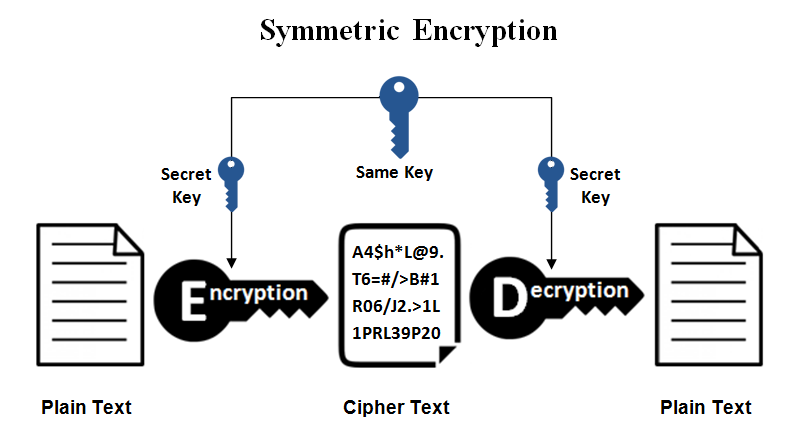
\includegraphics[width=.5\textwidth]{fig/Chapter-2/chapter-2/symmetric-encryption.png}}
\subfloat[][]{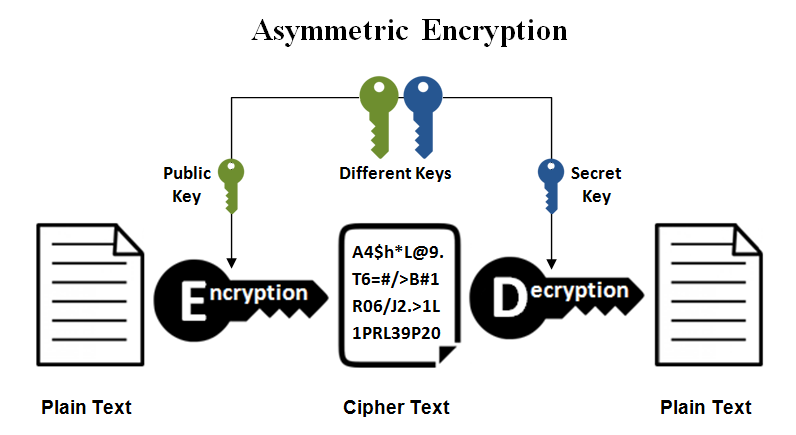
\includegraphics[width=.5\textwidth]{fig/Chapter-2/chapter-2/asymmetric-encryption.png}}

\caption{Cifratura simmetrica ed asimmetrica}\label{img:cifratura}
\end{figure}

Il \textbf{Quantum Computing} ha reso più vulnerabili gli odierni algoritmi di cifratura. Questo perché tali algoritmi basano la loro complessità sulla complessità computazionale molto elevata che viene richiesta per brute-forzare una chiave. In particolare:
\begin{itemize}
    \item \textbf{L'algoritmo di Shor}: Tale algoritmo permette di poter fattorizzare un numero intero in numeri primi è una minaccia importante per gli algoritmi a chiave asimmetrica. Tale algoritmo richiede molti qubit per essere eseguito, ma nonostante tutto è comunque potenzialmente pericoloso. Questo succede perché nella cifratura a chiave asimmetrica le chiavi che vengono utilizzare sono comunque collegate matematicamente
    
    \item \textbf{L'algoritmo di Grover}: Tale algoritmo permette di poter cercare un elemento all'interno di una lista con il brute force. Questo algoritmo può essere pericoloso per gli algoritmi a chiave simmetrica. 
\end{itemize}

Entrambe le soluzioni precedenti portano ad uno speed-up degli algoritmi per "bucare" tali sistemi. 

\begin{warn}
La comunità internazionale, accortasi del problema, in particolare per le comunicazioni asimmetriche, ha deciso di utilizzare degli algoritmo "\textbf{quantum-proof}" che sono stati chiamati algoritmi della \textbf{Post-Quantum Cryptography}, che invece cerca di sfruttare dei problemi matematicamente impossibili. O se non impossibili, non risolvibili ne da un computer classico ne da un computer quantistico
\end{warn}

\subsubsection{I fondamenti del QKD}
Il QKD cerca di sfruttare due fondamenti principali per la quantum information, ovvero:
\begin{itemize}
    \item Il teorema del \textbf{No-Cloning}
    \item Il \textbf{Postulato della Misura Quantistica}
\end{itemize}

Immaginiamo che Alice e Bob debbano comunicare tra di loro, vogliono sfruttare il QKD per distribuire la chiave simmetrica che poi andranno ad utilizzare per la loro comunicazione in modo classico. Pertanto quello che si va ad effettuare è sfruttare la misurazione su diverse coppie EPR, per poi scambiarsi le modalità di misura, da cui si decreterà poi la chiave (il metodo sarà esplorato meglio nelle prossime slide). La cosa importante è capire che per un eventuale attaccante che vorrà provare ad effettuare il man in the middle, sarà impossibile intromettersi all'interno di una comunicazione (non come nel mondo classico, dove con un cavo ethernet o con scheda wifi in modalità monitor, mediante wireshark, posso visualizzare i pacchetti letti dall'interfaccia, e provare ad effettuare attacchi di diverso tipo).

Se qualcuno provasse ad introdursi all'interno della comunicazione, non potrebbe farlo senza portare all'interno del sistema un disturbo. Questo è dimostrabile anche matematicamente come di seguito

\begin{info}
Per dimostrare che un man in the middle non possa entrare all'interno della comunicazione senza introdurre un disturbo, immaginiamo per assurdo che possa farlo. Pertanto ipotizzando che \(\ket{\psi}\) e \(\ket{\varphi}\) siano due stati non ortogonali su cui Eve(l'intruso) sta provando ad ottenere informazione. Di conseguenza, per non inserire disturbo, EVE effettuerà un'operazione unitaria tra \(\ket{\psi}\) o \(\ket{\varphi}\) con un'ancilla preparata in uno stato standard \(\ket{u}\). Assumendo che tale processo non disturbi gli stati, nei due casi si ottiene:
\[
\ket{\psi}\ket{u}\rightarrow \ket{\psi}\ket{v}
\]
\[
\ket{\varphi}\ket{u} \rightarrow \ket{\varphi}\ket{v'}
\]

Eve vuole che \(\ket{v}\) e \(\ket{v'}\) siano diversi per poter ricavare qualche informazione. Dato che il prodotto interno è preservato attraverso le trasformazioni unitarie, si va ad impostare la seguente uguaglianza:
\[
\braket{v | v'} \braket{\psi | \varphi} = \braket{u | u} \braket{\psi | \varphi}
\]

Essendo \(\ket{\psi}\) e \(\ket{\varphi}\) due vettori non ortogonali per ipotesi, allora \(\braket{\psi | \varphi} \ne 0\), il che mi permette di poterli ignorare da ambo le parti dell'equazione, ottenendo:
\[
\braket{v | v'} = \braket{u | u} = 1
\]
\end{info}

Questo implica che \(\ket{v}\) e \(\ket{v'}\) debbano essere lo stesso vettore, il che si traduce che Eve per ottenere informazione deve per forza introdurre disturbi all'interno della comunicazione.


\subsection{Bennett Brassard 1984 (BB84)}
Tale protocollo è il primo protocollo, che sfruttando il no-cloning, cerca di rendere possibile la condivisione di una chiave di cifratura classica mediante tecnologie quantistiche. I passi che si vanno a seguire sono i seguenti:

\begin{enumerate}
\item Alice genera una prima stringa di bit randomici di una lunghezza arbitraria (seguendo il riferimento \cite{nielsen2010}, \((4+\delta)n\), tale stringa di bit è denominata dal testo come \(a\))
\item Alice sceglie un'altra stringa di bit, che andranno a definire la base di riferimento (\(0:\{\ket{0}, \ket{1}\}\) oppure per \(1:\{\ket{+},\ket{-}\}\), tale stringa, nel testo, viene denominata \(a\))
\item Alice va a preparare, rispetto alle due precedenti stringhe, i qubit per la comunicazione. Precisamente il sistema potrà essere visto come:
\[
\ket{\psi} = \bigotimes_{k=1}^{(4+\delta)n} \ket{\psi_{a_k b_k}}
\]

Dove i singoli qubit \(\ket{\psi_{a_k b_k}}\) vegono preparati in base ai valori della stringa \(a\) e della stringa \(b\) seguendo la regola per cui:
\begin{itemize}
    \item \(a_k=0, b_k=0\): \(\ket{\psi_{00}}=\ket{0}\)
    \item \(a_k=1, b_k=0\): \(\ket{\psi_{10}}=\ket{1}\)
    \item \(a_k=0, b_k=1\): \(\ket{\psi_{01}}=\ket{+}\)
    \item \(a_k=1, b_k=1\): \(\ket{\psi_{11}}=\ket{-}\)
\end{itemize}
Una volta preparati, li invia direttamente a Bob

\item Bob riceve i qubit inviati da Alice e lo annuncia (tipo un piccolo ack di ricezione). Una volta fatto questo, Bob procede a misurare i qubit seguendo le indicazioni di una stringa randomica che genera esso stesso (tale stringa, nel testo viene chiamata \(b'\))
\item Alice annuncia la stringa \(b\)
\item Bob annuncia la stringa \(b'\) (questa non viene citata nel testo, ma è necessaria per il funzionamento del protocollo)

\item Alice e Bob scartano ogni bit che Bob ha misurato con una base differente da quella con cui alice aveva preparato i qubit. Con una probabilità abbastanza alta, ci sono almeno \(2n\) bit mancanti (se non dovesse essere così, allora si interrompe il protocollo). Loro manterranno \(2n\) bit
\item Alice seleziona un sottoinsieme di \(n\) bit che andrà ad utilizzare per verificare se ci sia una interferenza portata da Eve, per poi dire a bob quali bit ha selezionato
\item Alice e Bob annunciano e comparano i valori degli n bit di check. Se più di un certo numero accettabile, sono diversi, allora si termina il protocollo
\item Alice e bob faranno una riconciliazione e un amplificazione di privacy sui restanti \(n\) bit per ottenere \(m\) chiavi condivise.
\end{enumerate}

Quello che accade dal passo 7 in poi è una verifica per comprendere se Eve ha introdotto più disturbo (rispetto anche a quello introdotto dall'eventuale canale tra Alice e Bob). Questo avviene selezionando un sottoinsieme dei bit che sono stati "concordati" tra i due, verificato che tali bit differiranno per una valore determinato di t bit. Tale verifica permetterà di capire se Eve si è introdotta con ulteriore disturbo o meno. 

Il difetto del BB84 è che, sfruttando l'invio dei qubit, richiede un'infrastruttura apposita. Precisamente, richiede dei trusted node su cui ci si ferma ad effettuare il protocollo per poi generare una serie di comunicazioni tra i trusted node fino a destinazione. Il motivo è dovuto al fatto che un fotone, nel mondo quantistico, per via del no-cloning, non può essere rigenerato, come nel modo classico, da un normale ripetitore.

\subsection{Ekert 1991 (E91)}
L'Ekert 1991 (o Ekert-91 o E91) è un'estensione del protocollo QKD con l'utilizzo di coppie EPR. Quello che principalmente cambia è la trasmissione dei qubit stessi.

Le regole dell'Ekert-91 sono semplici:
\begin{enumerate}
    \item Alice e Bob pre-distribuiscono delle coppie EPR tra di loro
    \item Alice e Bob scelgono randomicamente le basi lungo cui misurare i loro qubit delle coppie EPR (generazione di due stringhe randomiche per la scelta delle basi, sono esattamente \(b\) e \(b'\) incontrate nel BB84)
    \item Alice e Bob si condividono le stringhe che spiegano lungo che base hanno effettuato la misura (si condividono \(b\) e \(b'\))
    \item Dopo la condivisione, Alice e Bob mantengono solo i bit che corrispondono alla stessa misura, questo ne permette la perfetta generazione della chiave
\end{enumerate}


\subsection{Considerazioni sul QKD}
Il QKD, come visto precedentemente, richiede:
\begin{itemize}
    \item Nel caso del BB84, di dover trasmettere dei fotoni lungo delle linee. Essendo che i fotoni, all'interno delle fibre, vengono persi (su 10 fotoni, solo uno arriva a destinazione dopo 50 km, gli altri vengono perduti)
    \item Nel caso dell'E91 è la distribuzione di molte coppie EPR tra trasmettitore e ricevitore. Essendoci anche la tecnica di quantum swapping, questo non è complicato, ma richiederebbe la realizzazione di porte in tecnologia fotonica (non proprio facili da realizzare)
\end{itemize}

Nelle implementazioni reali, però, bisogna tenere conto di:
\begin{itemize}
    \item Rumorosità del canale quantistico
    \item Eavesdropper (rumore introdotto da Eve)
\end{itemize}

Con la presenza di tali problematiche, la chiave che Alice e Bob vogliono condividere può contenere dei mismatch non dovuti al protocollo, ma dovuti ai diversi rumori. Essendo che Alice e Bob non possono rivelare le loro chiavi (per ovvi motivi), l'unico modo è utilizzare delle specifiche tecniche di post-processing. Tra queste troviamo:
\begin{itemize}
    \item \textbf{Key sifting}: rivelare alcune delle chiavi condivise
    \item \textbf{Key reconciliation}: correzione dell'errore sulla chiave setacciata
    \item \textbf{Privacy amplification}: riduzione della chiave setacciata
\end{itemize}

\subsubsection{Key Sifting}
La tecnica del Key Sifting permette di capire l'entità dell'informazione che è stata "perduta" o disturbata durante la trasmissione. Questo avviene con la condivisione di parte della chiave che viene condivisa per essere confrontata. Una volta confrontata si decide se arrestare il protocollo in base al BER(Bit Error Rate) threshold. In particolare:
\begin{itemize}
    \item Se: BER osservato < BER threshold -> si può procedere con la key reconciliation
    \item Se: BER osservato >= BER threshold -> bisogna interrompere il protocollo, potenziale eavesdropper
\end{itemize}

Non è possibile distinguere, solo dal BER, se vi è la presenza di eavesdropper o meno, questo perché il disturbo non viene distinto da quello introdotto dal canale di comunicazione stesso

\subsubsection{Key Reconciliation}
Quello che viene fatto in questa fase è cercare di ridurre il numero di mismatch della chiave tra Alice e Bob. Per effettuare questa cosa vi è una problematica, condividere la chiave su un canale non sicuro risulta impossibile. Pertanto quello che si va ad effettuare è la suddivisione in blocchi della chiave ed il calcolo della parità tra di loro. Trovati i mismatch, si vanno a scambiare solo tali mismatch, dove la parità è diversa. 

Quello che solitamente si va ad effettuare è un mescolamento dei bit con un'applicazione di \(k\) volte il check di parità (seguendo queste chiavi mescolate). Questo permette di poter evitare casi in cui la sola parità non basti. Aumentando considerevolmente il numero di \(k\), la probabilità che le chiavi siano identiche aumenta (perché si riduce la probabilità di "errori nascosti").

La probabilità di errori nascosti si esprime come:
\[
p = 1 - \left(\frac{1}{2}\right)^k
\]
Tale tecnica non è molto difficile da implementare, ma questo non basta, essa ha anche dei contro che sono:
\begin{itemize}
    \item Quantità gigante di informazioni che trapelano su di un canale non sicuro
    \item delay molto grande per la correzione dell'errore
\end{itemize}

La soluzione a tali problemi risiede nell'utilizzare metodologie di error-correction più forti, come ad esempio: Turbo codes, LDPC codes, Polar codes.

\subsubsection{Privacy Amplification}
La key reconciliation è un'operazione che avvenendo su un canale non sicure, rende i "messaggi" si comunicazione tra Alice e Bob visibili, il che aggiungerà informazioni utili ad Eve per "decifrare" la chiave. Quindi Alice e Bob hanno bisogno di eliminare quanta più informazione sporcata, sia da Eve, che da eventuale rumore.

Bisogna quindi trovare il modo di effettuare delle operazioni di \textbf{Privacy Amplification}.
Assumendo che Alice e Bob condividano n-bit della chiave condivisa ed Eve ha t-bit della chiave ricavati (Alice e Bob non hanno idea di quali t bit siano). La domanda che quindi ci si pone è: è possibile che Alice e Bob possano usare la chiave corrente? Hanno bisogno di ricominciare il processo da capo?

Non è necessario ricominciare il processo. Alice e Bob possono generare una chiave segreta di (n-t) bit a partire dalla chiave condivisa di n bit. Pur non sapendo quali bit siano noti a Eve, possono stimare approssimativamente quanti sono (t). Applicano allora una funzione hash universale, scelta a caso e comunicata pubblicamente, che comprime la chiave mescolandone tutti i bit: la chiave risultante, più corta, è segreta per Eve e può essere usata per la cifratura


\chapter{Quantum Noise}
Quando si parla di \textbf{Quantum Noise}(o rumore quantistico) è una tipologia di rumore che va ad intaccare lo stato del mio qubit. Come abbiamo visto precedentemente, lo stato di un qubit è definibile come:

\begin{gather*}
\ket{\psi} = \alpha \ket{0} + \beta \ket{1}\\
|\alpha|^2 + |\beta|^2 = 1
\end{gather*}

Con tale dfeinizione, lo stato, se ad esempio fosse:
\begin{gather*}
\ket{\psi} = \ket{0}
\end{gather*}

Se misurassi lungo \(Z\), otterrei uno stato determinato deterministicamente. Mentre, se vi è rumore, questo non è detto. Questo vuol dire che lo stato non è ben definito.

a definizione che si tende a dare è quella di \textbf{stato misto}. Per stato misto si intende uno stato di un sottoinsieme del sistema che si sta osservando. Quindi non si sta più generalizzando il sistema ad un sistema chiuso di n-qubit, ma si sta andando a considerare tale sistema come parte di un sistema più grande. Come se si fossero "ricollegati" con la realtà i Qubit. Tale approccio mostra come si ci potrebbe trovare in casi in cui lo stato di un Qubit "entri" nella sfera di Bloch e non si muova più solo sulla superfice.

La conoscenza di tutti gli stati misti di un sistema non implica la conoscenza dello stato del sistema intero; questo è vero solo dal momento in cui si sà che non ci sono coppie di qubit entangled tra di loro.

Quindi, si può parlare di stato misto poichè, iniziando a decadere l'ipotesi di sistema chiuso, allora il qubit inizierà ad interagire con l'ambiente, diventando a tutti gli effetti una \textbf{parte} di un sistema più complesso. Quindi una sottoparte \cite{gentle2011quantum}.

Di conseguenza, gli stati non saranno più puramente deterministici e sarà quindi possibile definire una probabilità di trovarsi in uno stato puro \(p_i\), andando a definire la coppia:
\[
\{(p_i,\ket{\psi_i})\}
\]
Dove \(p_i\) è la probabilità di trovarsi nello stato puro \(\ket{\psi_i}\).

\section{Density Operator}
Prima di affrontare il discorso legato al \textbf{density operator} è importante approfondire quella che è una matrice di proiezione.

\begin{info}
\textbf{Projection Operator}\\
Una proiezione su uno spazio vettoriale \(\mathbb{V}\) è un operatore lineare \(P:\mathbb{V} \rightarrow \mathbb{V}\) tale per cui \(P^2=P\).
Se \(\mathbb{V}\) è uno spazio di Hilbert, può essere utilizzato il concetto di ortogonalità. Una proiezione \(P\) su uno spazio di Hilbert \(\mathbb{V}\) è detta ortogonale se soddisfa la seguente proprietà:
\[
<P x,y> = <x,P y>, \forall x,y \in \mathbb{V}
\]
Una proiezione sullo spazio di Hilbert che non è ortogonale è chiamata anche \textbf{proiezione obliqua}(citata solo 
per conoscenza e completezza).\\
\\
\textbf{Matrice di Proiezione}\\
La matrice di proiezione è una matrice quadrata che gode della proprietà elencata prima, ovvero: \(P^2=P\) (dove il prodotto tra due matrici è il prodotto riga per colonna).
Si definisce anche \textbf{matrice di proiezione ortogonale} se: \(P^2=P=P^T\) nel caso di spazi vettoriali reali, mentre nel caso di spazi vettoriali complessi si avrà \(P^2 = P = P^\dagger\).

Se la matrice di proiezione non è una matrice di proiezione ortogonale allora si dice \textbf{matrice di proiezione obliqua}.

Una conseguenza delle matrici di proiezione che sono matrici di proiezione ortogonale è che tutti gli autovalori associati saranno 1 e 0 con diversi gradi di molteplicità algebrica
\end{info}


L'\textbf{operatore di densità} è un modo alternativo di rappresentare gli stati e di formulare i postulati della meccanica quantistica. Tale strumento permette di poter esprimere meglio la gestione di alcuni scenari comuni nella meccanica quantistica. Una delle cose principali da capire è l'\textbf{ensembles of quantum states} (insiemi di stati quantistici), tale teoria ha come base quello presentato nella precedente sezione, ovvero, che uno stato quantistico non è detto sia puro, poichè non sarà possibile avere a propria disposizione lo stato di tutto il sistema, ma sarà misto, e quindi, confinato ad uno specifico sottositema. Dati quindi, gli stati \(\ket{\psi_i}\) in cui il sistema può trovarsi e \(p_i\) probabilità di trovarsi nell'\(i\)-esimo stato. Si chiamerà insieme di stati puri il duo: \(\{p_i,\ket{\psi_i}\}\). L'operatore di densità (o matrice di densità), sarà quindi definibile come:
\begin{gather*}
\rho = \sum_{i} p_i \ket{\psi_i} \bra{\psi_i}
\end{gather*}

Con tale definizione sarà possibile andare a riformulare anche quelli che sono i postulati stessi della meccanica quantistica, andando a spiegare anche quando tale notazione sia utile. 

\subsubsection{Legge di Shrodinger}
Quella che deriva dal quarto postulato della meccanica quantistica spiegando che l'evoluzione di un sistema quantistico è definito da matrici unitarie. Definendo quindi l'operatore unitario \(U\), considerando che inizialmente lo stato è \({p_i, \ket{\psi_i}}\), allora applicando l'evoluzione unitaria si avrà:
\(\ket{\psi_i} \rightarrow U \ket{\psi_i}\), dove la probabilità non è cambiata, quindi il nuovo stato sarà definito come: \(\{p_i, U \ket{\psi_i}\}\), quindi la probailità non cambia, andando ad analizzare quello che succede matematicamente, si avrà:

\begin{gather*}
\rho=\sum_{i} p_i \ket{\psi_i}\bra{\psi_i} \overset{U}{\longrightarrow} \sum_{i} p_i U \ket{\psi_i}\bra{\psi_i}U^\dagger = U \rho U^\dagger
\end{gather*}

\subsubsection{Postulato della misura}
Il postulato della misura è descrivibile mediente il linguaggio dell'operatore di densità. Supponiamo di effettuare una misurazione descritta da un operatore di misura \(M_m\). 

\begin{info}
\textbf{Proiettori degli autostati}\\
Dato un osservabile A ed i suoi autostati \(\{\ket{a_j}\}\) si introducono i proiettori su tali autostati come:
\begin{gather*}
M_j = \ket{a_j}\bra{a_j}
\end{gather*}

Un proiettore si dice \textbf{Hermitiano idempotente} quando soddisfa la proprietà tale per cui:
\begin{gather*}
P^2=P=P^\dagger
\end{gather*}

Queste sono esattamente le proprietà presentate precedentemente per l'operatore di densità ortogonale (Hermitiano + Idempotente).

Nei nostri casi, ad esempio, misurando l'osservabile \(Z\), i cui autostati sono \(\{\ket{0},\ket{1}\}\), si avrà che sarà possibile definire i seguenti due proiettori:
\begin{gather*}
M_0 = \ket{0}\bra{0} =
\left[\begin{smallmatrix}
1 & 0 \\
0 & 0
\end{smallmatrix}\right] \\
M_1 = \ket{1}\bra{1} =
\left[\begin{smallmatrix}
0 & 0 \\
0 & 1
\end{smallmatrix}\right]
\end{gather*}

Come visto anche in precedenza, essendo tale operatore ortonormale si avrà che i suoi autovalori saranno 0 ed 1.

Date queste nozioni, sarà quindi definibile come proiettore, un operatore unitario che aisce su un vettore di uno spazio vettoriale di Hilbert \(\mathcal{H}\) di dimensione \(N\), trasformandolo nella sua componente appartenente ad un sottospazio \(\hat{\mathcal{H}} \in \mathcal{H}\) di dimensione \(M\). Sia \(\{\ket{1}, \ket{2}, \dots, \ket{N}\}\) una base ortonormale di \(\mathcal{H}\) e sia \(\hat{\mathcal{H}}\) il sottospazio generato dai vettori \(\{\ket{1}, \ket{2}, \dots, \ket{M}\}\), il proiettore su tale stato è:
\begin{gather*}
P=\sum_{i=1}^{M} \ket{j}\bra{j}
\end{gather*}

Un operatore \(M\) è detto \textbf{normale} se: \(M M^\dagger = M^\dagger M\). Ma gli operatori unitari godono della proprietà per cui: \(U U^\dagger = I = U^\dagger U\). 

Gli operatori normali giocano un ruolo fondamentale per il teorema della decomposizione spettrale. Ogni operatore normale \(M\) su un vettore \(V\) è diagonale rispetto a qualche base ortogonale per \(V\). Di conseguenza, ogni operatore diagonalizzabile è normale. Questo significa che \(M\) può essere scritto come \(M=\sum_{i} \lambda_i \ket{i}\bra{i}\) dove i \(\lambda_i\) sono gli autovalori di \(M\), \(\{\ket{i}\}\) è una base ortogonale per \(V\), e ogni \(\ket{i}\) è un autovettore di \(M\) con autovalore \(\lambda_i\). Tali proiettori soddisfano la relazione di completezza, ovvero:
\begin{gather*}
\sum_{i} P_i = I
\end{gather*}
\end{info}

\begin{info}
L'uguaglianza segue dalla definizione di traccia,
$\operatorname{tr}(B)=\sum_k \bra{k}B\ket{k}$, calcolata in una base
ortonormale $\{\ket{k}\}$, e dalla relazione di completezza
$\sum_k \ket{k}\bra{k}=I$. Posto $A=M_m^\dagger M_m$, si ha
\begin{align*}
\operatorname{tr}\left(A\ket{\psi_i}\bra{\psi_i}\right)
  &= \sum_k \bra{k}A\ket{\psi_i}\braket{\psi_i | k} \\
  &= \sum_k \braket{\psi_i|k}\bra{k}A\ket{\psi_i} \\
  &= \bra{\psi_i}\Big(\sum_k \ket{k}\bra{k}\Big)A\ket{\psi_i}
   = \bra{\psi_i}A\ket{\psi_i},
\end{align*}
dove nel secondo passaggio si sono scambiati due scalari. Equivalentemente,
è un'applicazione della ciclicità della traccia,
$\operatorname{tr}(XY)=\operatorname{tr}(YX)$, con $X=A\ket{\psi_i}$ e
$Y=\bra{\psi_i}$, tenendo conto che la traccia di uno scalare è lo scalare
stesso.
\end{info}

Laprobabilità che, quindi, misurando l'osservabile \(A\) a partire dallo stato \(\ket{\psi}\) il sistema si porti nello stato \(\ket{a_j}\) è data da:
\begin{gather*}
p_j=Tr\left(M_j\rho\right)
\end{gather*}

La dimostrazione di tale proprietà è una conseguenza diretta:
\begin{gather*}
Tr\left(M_j\rho\right) = \sum_{k}\bra{a_k}M_j \rho \ket{a_k} = \sum_{k}\bra{a_k}\ket{a_j}\bra{a_j}\ket{\psi}\bra{\psi}\ket{a_k} =\\
=b_j b_j^* = |b_j|^2
\end{gather*}

Dove il termine \(\bra{a_k} \ket{a_j} \ne 0 \iff k=j\), e quindi, dato che siamo con una base ortonormale, \(\bra{a_k} \ket{a_k} = 1\), di conseguenza si avrà:
\begin{gather*}
\bra{a_k} \ket{\psi} \bra{\psi} \ket{a_k} = b_k b_k^* = |b_k|^2
\end{gather*}
Dato che stiamo andando a filtrare la \(k\)-esima componente del vettore \(\ket{\psi}\) mappata sul autovettore \(\ket{a_k}\). Ottenendo di conseguenza la relazione.

\subsubsection{Caratteristiche del density operator}
Il density operator gode di diverse proprietà:
\begin{itemize}
       \item \(\rho\) è Hermitiano, quindi: \(\rho = \rho^\dagger\)
       \item Traccia unitaria: \(Tr(\rho) = 1\)\\
       Tale proprietà è dimostrabile mediantei seguenti passaggi:
       \[
       Tr(\rho) = \sum_{k} \bra{k} \rho \ket{k} = \sum_{k} \sum_{i} p_i \bra{k}\ket{\psi_i}\bra{\psi_i}\ket{k} =
       \sum_{i}p_i \bra{\psi_i} \sum_{k}\ket{k}\bra{k}\ket{\psi_i} =
       \sum_{i}p_i = 1
       \]
       o equivalentemente:
       \[
       Tr(\rho) = Tr(\sum_{i}p_i\ket{\psi_i}\bra{\psi_i})=
       \sum_{i}p_i Tr(\ket{\psi_i}\bra{\psi_i})=
       \sum_{i} p_i = 1
       \]

       \item \(\rho\) è semidefinito positivo, ovvero:
       \[
       \bra{\psi}\rho\ket{\psi} \ge 0, \forall \ket{\psi}
       \]
       Tale proprietà discende dal fatto che gli autovalori di \(\rho\) sono tutti reali (essendo \(\rho\) Hermitiano) e non-negativi, quindi dalla condizione: \(Tr(\rho) = 1, 0 \le \lambda_i \le 1\).

       La dimostrazione di tale proprietà discende dalla definizione data precedentemente:
       \[
       \bra{\varphi}\rho\ket{\varphi} = \sum_{i}p_i\braket{\varphi | \psi_i}\braket{\psi_i | \varphi}=\sum_{i} p_i |\braket{\varphi | \psi_i}|^2 \ge 0
       \]
       Dato che \(p_i\) essendo una probabilità non potrà essere mai zero. Lo stesso valer per il modulo del numero complesso ottenuto.

       Se supponiamo che \(\rho\) è un operatore che soddisfa le condizioni di traccia e di positività, si avrà che:
       \[
       \rho=\sum_{j}\lambda_j \ket{j}\bra{j}
       \]
       dove i vettori \(\ket{j}\) sono ortogonali e i \(\lambda_i\) sono autovalori reali e non-negativi di \(\rho\).
\end{itemize}

Per uno stato puro \(\ket{x}\), l'operatore di densità \(\rho_x^X=\ket{x}\bra{x}\) ha una forma perticolarmente semplice. Se consideriamo che \(\ket{x}\) è l'i-esimo elemento di una base ortonormale, allora \(\ket{x}\) è il vettore della base con tutti 0 ed un solo 1 nella i-esima posizione. Di conseguenza, il prodotto \(\ket{x}\bra{x}\) sarà uguale ad una matrice composta da tutti 0 e con un solo 1 presente sulla diagonale alla posizione \(ii\). Segue quindi la proprietà che l'operatore di densità di uno stato puro è un proiettore di quest'ultimo, ovvero: \(\rho_x^X \rho_x^X = \rho_x^X\). Contrariamente, ogni operatore di densità che è un proiettore corrisponde ad uno stato puro: operatori di proiezione hanno solo 0 ed 1 come autovalori, e per ottenere la traccia uguale ad 1, l'operatore di densità avrà un solo ed unico autovettore, che corrisponderà allo stato puro di quell'operatore.

Nel caso in cui mi trovi in degli stati misti, invece, l'operatore di densità, sulla diagonale, non avrà tutti 1 e 0, questo si dice che lo stato si un misto di diversi stati puri nell'insieme per \(\rho\). Uno stato puro, quindi, soddisfa il criterio per cui \(tr(\rho^2)=1\) questo perchè avendo un solo 1 sulla diagonale, il risultato è "ovvio". Mentre nel caso in cui ci sia uno stato misto, si avrà che \(tr(\rho^2) < 1\), questo perchè la somma degli autovalori \(\lambda_j\) sulla diagonale è uguale ad 1, ma questo impone che tali valori siano \(0 \le \lambda_j \le 1\), di conseguenza si avrebbe che la traccia sia definita come: \(Tr(\rho^2)=\sum_{i}\lambda_i^2 < 1\). Quindi, dato un operatore di densità \(\rho\), la decomposizione \(\rho=\sum_{i} p_i \ket{\psi_i}\bra{\psi_i}\) non è unica. 


% % Roba Vecchia
% si definisce come:
% \[
% \rho = \sum_{i} p_i \ket{\psi_i}\bra{\psi_i}
% \]

% Dove il termine \(\rho\) incapsula all'interno della sua struttura sia la probabilità dello stato puro \(p_i\) che lo stato puro stesso \(\ket{\psi_i}\).
% Per un sistema, invece, dove non andiamo a considerare una sua restrizione, ma un suo stato puro, si avrà:
% \[
% \rho = \ket{\psi}\bra{\psi}
% \]
% E tutti i postulati della meccanica quantistica possono essere espressi in termini di operatori di densità








\chapter{Quantum Error Correction}
Connettere tra loro più dispositivi quantistici richiede l'utilizzo di una rete quantistica. Tali collegamenti hanno un impatto fondamentale su diverse aree della Quantum Information, come:
\begin{itemize}
    \item Distribuited Quantum Computing
    \item Blind Quantum Computing
    \item Secure Classical Communication
    \item Quantum secret-sharing
    \item Molte altre applicazioni possibili
\end{itemize}

Ma questo richiede uno scambio di informazione quantistica tra i diversi dispositivi. Come visto precedentemente tale cose non è proprio facile, dato il teorema del no-cloning. Questo pone, quindi, la quantum teleportation e la quantum error correction al centro del dibattito generale. Tali tecnologie utilizzano tra di loro l'entanglement che viene "distribuito" tra i diversi dispositivi. La distribusione, fisicamente, ad oggi, avviene mediante l'utilizzo di fibre ottiche che trasportano fotoni (che possono essere entanglati anche con altre particelle). In generale la distribuzione delle coppie EPR è rumorosa (come anche nel caso classico), questo porta alla definizione dei \textbf{Canali Quantistici}.

Il modello associato ad un canale quantistico è definito a partire dalla matrice di densità \(\rho = \ket{\psi}\bra{\psi}\) del sistema che viene "elaborata" seguendo la seguente definizione:
\begin{gather*}
    \mathcal{N}(\rho) = \sum_i N_i \rho N_i^\dagger
\end{gather*}

Tale definizione può essere fatta (per il teorema di Kraus) solo se la funzione è lineare CPTP(Completamente Positivo e Traccia Preservante). L' \(\{N_i\}\) è un insieme di operatori di Kraus che soddisfano il criterio di completezza:

\begin{gather*}
    \sum_i N_i^\dagger N_i = I
\end{gather*}

Da tale definizione generale è possibile andare a definire anche il modello di Pauli del canale, dato da:
\begin{gather*}
    \mathcal{N}(\rho) = \sum_{i=0}^3p_i \sigma_i \rho \sigma_i^\dagger
\end{gather*}

Dove, \(p_i\) è la probabilità che avvenga un errore di tipo \(i\) (dove \(0\rightarrow I\), \(1 \rightarrow X\), \(2 \rightarrow Y\), \(3 \rightarrow Z\)). Le matrici \(\sigma_0 = I, \sigma_1 = X, \sigma_2=Y, \sigma_3 = Z\). Se volessimo valutare l'insieme di operatori di Kraus associati a tale modello, si avrebbe \(N_i = \sqrt{p_i}\sigma_i\). 

Dalla definizione del canale di Pauli è possibile definire anche il canale di depolarizzazione quantistica, dove, alla fine, sì ha che tutti i possibili errori di pauli sono equiprobabili, per cui il canale sarà definibile come:
\begin{gather*}
    \mathcal{N}(\rho) = (1-p)\rho + \frac{p}{3}(X \rho X^\dagger + Y \rho Y^\dagger + Z \rho Z^\dagger)
\end{gather*}

Dove la \(p\) denota la probabilità di depolarizzazione. 

Solitamente andare a studiare tali canali risulta molto oneroso, pertanto si vanno a considerare dei canali ridotti, che vanno ad isolare i singoli errori. I canali maggiormente utilizzati sono:
\begin{itemize}
    \item \textbf{Quantum Bit-Flip Channel}: \(\mathcal{N}(\rho) = (1-p)\rho + p X \rho X\)
    \item \textbf{Quantum Phase-Flip Channel}: \(\mathcal{N}(\rho)=(1-p)\rho + p Z \rho Z\)
\end{itemize}

Tali errori possono essere visualizzati mediante delle deformazioni che il canale effettua sulla sfera di Bloch stessa. L'unico valore che non viene toccato della sfera di Bloch è quello dell'errore stesso. Ad esempio nell'errore di tipo X, i valori su tale asse non cambiano. I restanti assi, invece, si contraggono di una quantità definita da \((1-2p)\). Data tale condizione, quindi, sarebbe utile andare a mappare le informazioni sull'asse che meno viene impattato dal canale, in modo da poter evitare la decoerenza. Quest'asse va a definire un sottospazio tutto suo, definito come \textbf{Decoherence Free Subspace}. Le possibili deformazioni della sfera di Bloch sono mostrate nelle figure [\ref{img:bloch-phase-flip}][\ref{img:bloch-bit-flip}][\ref{img:bloch-bit-phase-flip}]. 

\begin{figure}[H]
\centering
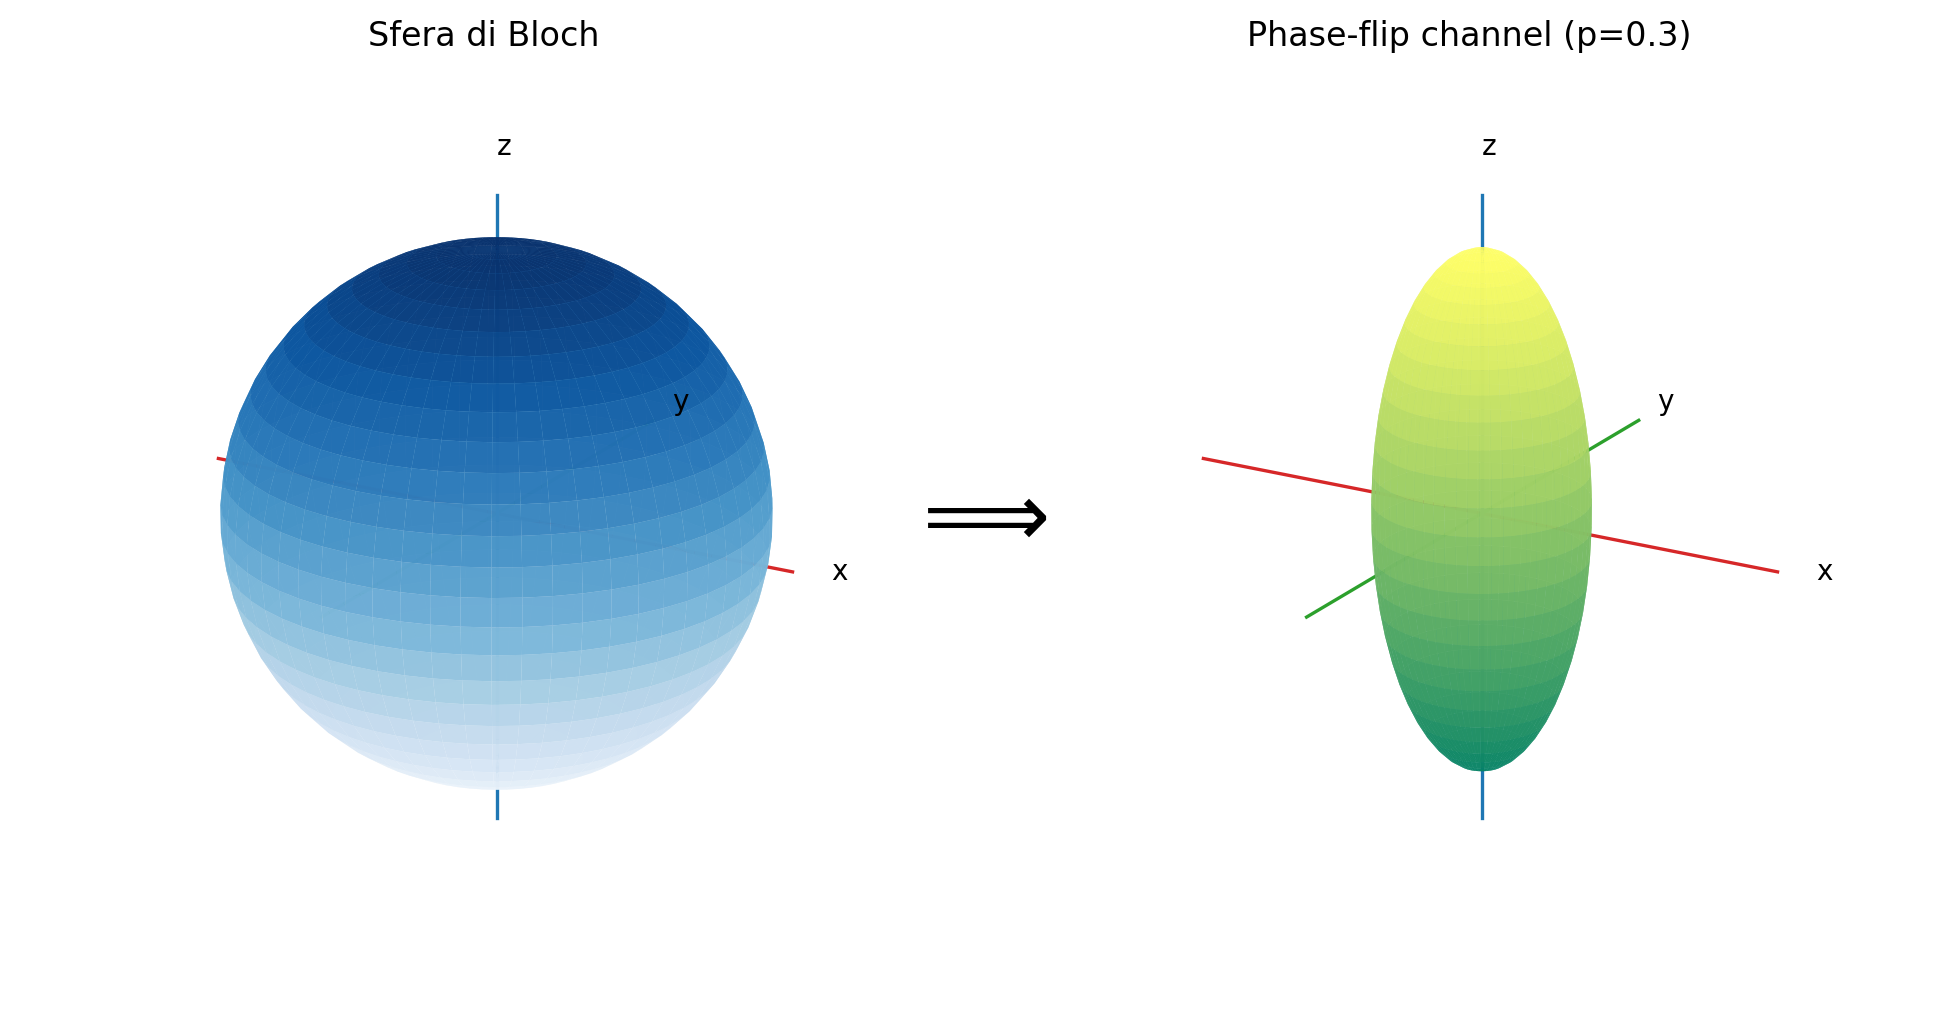
\includegraphics[width=.7\textwidth]{fig/Chapter-4/phase_flip.png}
\caption{Z Phase Flip}\label{img:bloch-phase-flip}
\end{figure}

\begin{figure}[H]
\centering
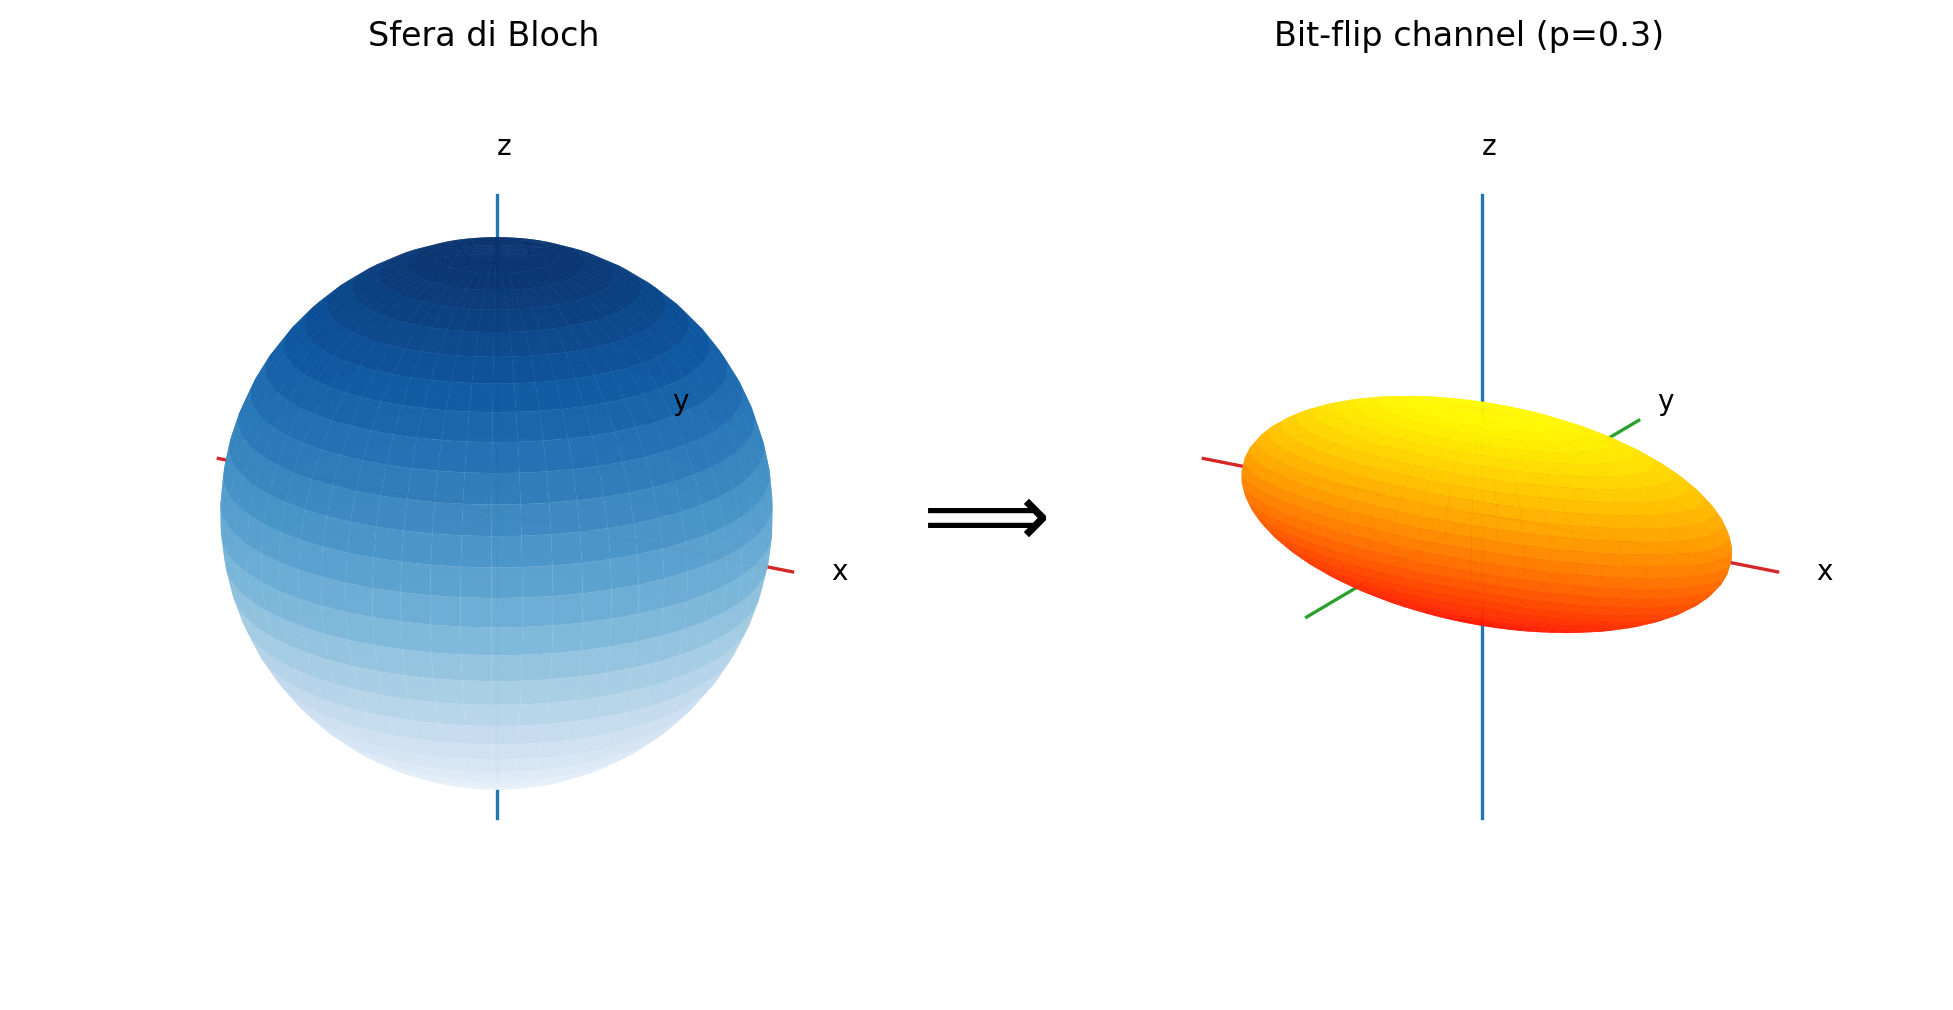
\includegraphics[width=.7\textwidth]{fig/Chapter-4/bit_flip.png}
\caption{X Bit Flip}\label{img:bloch-bit-flip}
\end{figure}

\begin{figure}[H]
\centering
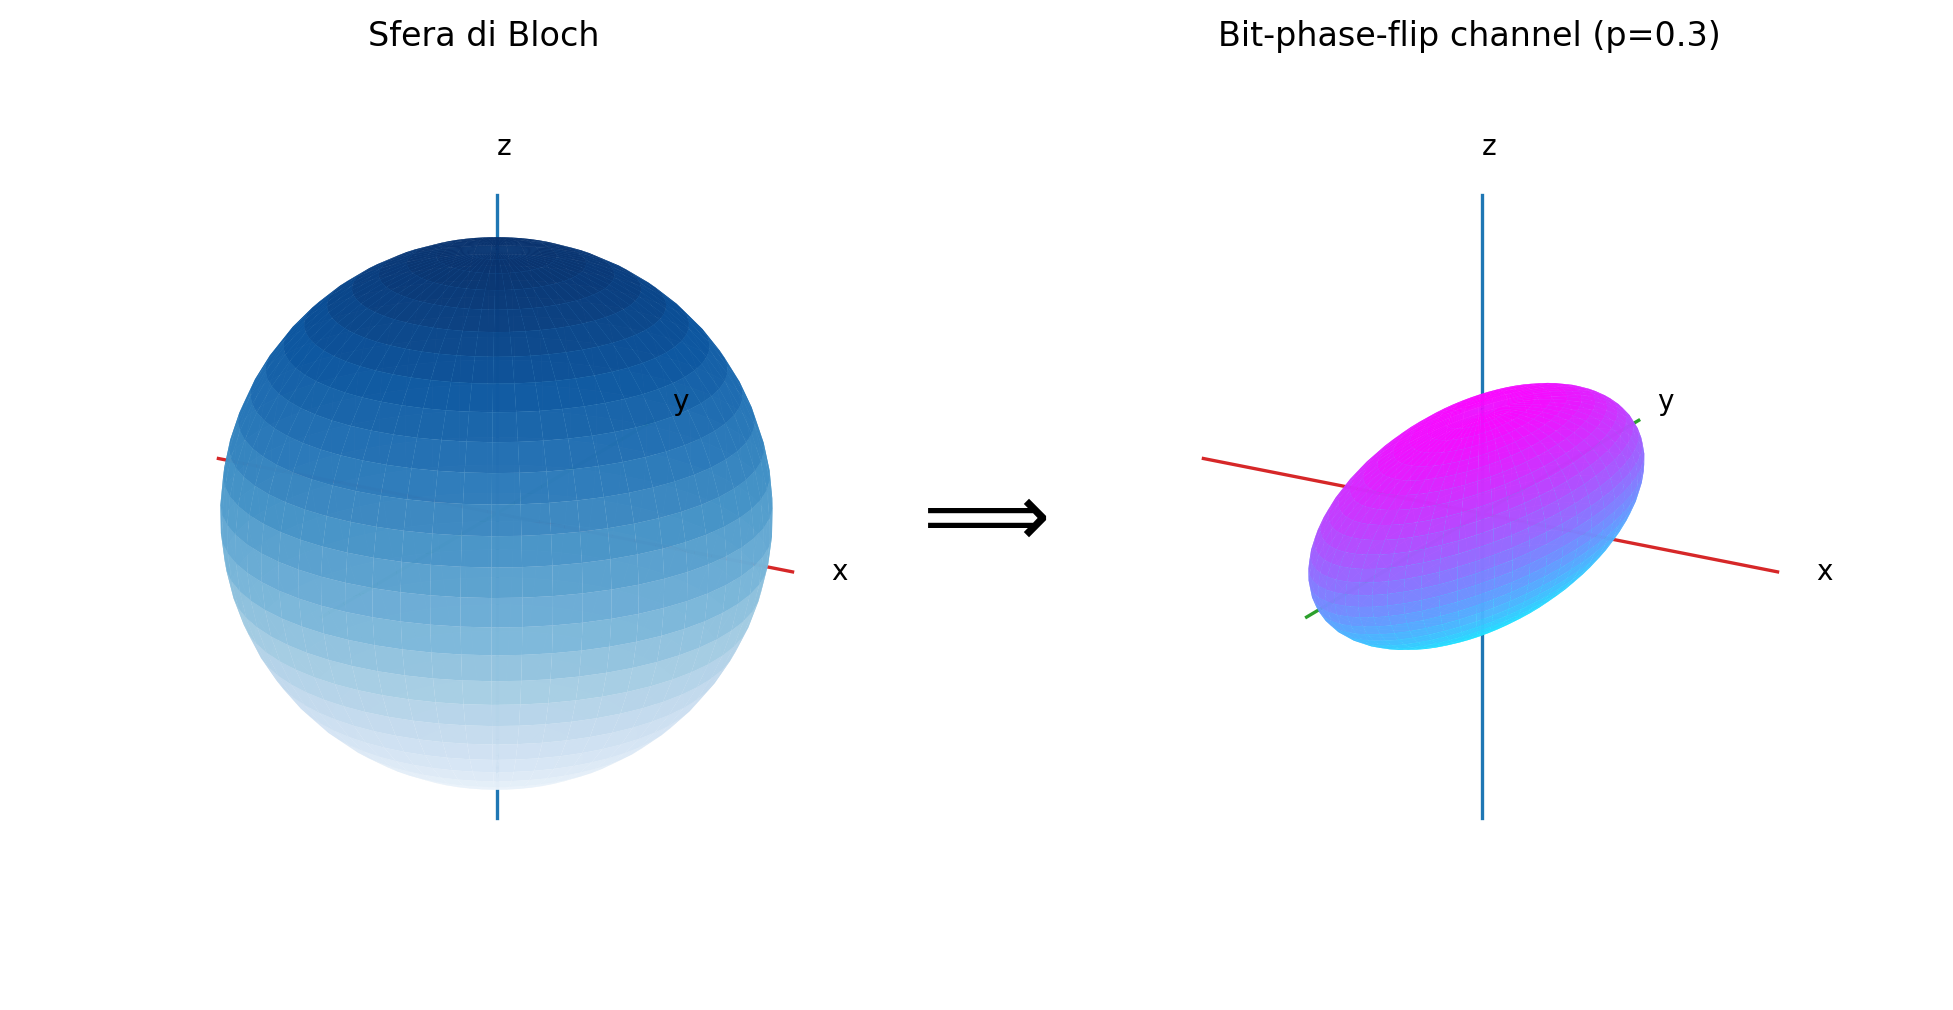
\includegraphics[width=.7\textwidth]{fig/Chapter-4/bit_phase_flip.png}
\caption{Y Pahse + Bit Flip}\label{img:bloch-bit-phase-flip}
\end{figure}

Nonostante la presenza di tali disturbi le coppie EPR rimangono coppie EPR, ma in un diverso stato di Bell. Se consideriamo come stato di partenza lo stato \(\ket{\Phi^+}_{AB} = \frac{1}{\sqrt{2}}(\ket{00}_{AB} + \ket{11}_{AB})\), avremo che, i diversi canali di Pauli presentati prima, agiranno nel seguente modo:
\begin{itemize}
    \item \textbf{Phase Flip Channel}: \(Z_A \ket{\Phi^+}_{AB} = \ket{\Phi^-}_{AB} = \frac{1}{\sqrt{2}}(\ket{00}_{AB} - \ket{11}_{AB})\)
    \item \textbf{Bit Flip Channel}: \(X_A \ket{\Phi^+}_{AB} = \ket{\Psi^+}_{AB} = \frac{1}{\sqrt{2}}(\ket{01}_{AB} + \ket{10}_{AB})\)
    \item \textbf{Y Channel}: \((XZ)_A \ket{\Phi^+} = \ket{\Psi^-}_{AB} = \frac{1}{\sqrt{2}}(\ket{01}_{AB} - \ket{10}_{AB})\)
\end{itemize}

\section{Quantum Error Correction}
Quando si parla di tecniche di error correction (che sia in caso quantistico o classico), si sta parlando di tecniche utilizzate per identificare e correggere l'errore. Nel mondo classico vi sono diverse tecniche che permettono di fare \textbf{error detection}(detectare l'errore) ed \textbf{error correction}. Una di queste è il codice a ripetizione che è stato esteso anche al caso quantistico. Pertanto gli si da una breve paronamica.

\subsection{Codice a ripetizione}
Dato un canale rumoroso, nel mondo classico, quello che può accadere è il fenomeno del bit flip. Quindi un bit quando viene inviato, al ricevitore, viene flippato dal canale stesso. Quindi da 0 diventa 1 o il vicevera.
Per modellare un sistema che permetta di essere "resistente" al canale si è pensato di poter replicare l'informazione più volte in modo che il ricevitore, anche nel caso di qualche bit flip, possa riconoscere l'informazione originale. Dalla teoria dell'informazione si dice che è possibile arrivare ad una probabilità di errore piccola a picere andando ad aumentare il numero di repliche dell'informazione (tale tecnica viene anche da una nostra predisposizione naturale, quando qualcuno non capisce qualcosa che gli stiamo dicendo, tendiamo a ripeterla più volte). Una delle tecniche più semplici è il \textbf{codice a ripetizione}. Un codice a ripetizione è un codice che va ad aumentare il numero di bit inviati per la singola informazione. Per esempio, se voglio inviare 0, lo invierò 3 volte (\(0 \rightarrow 000\)), lo stesso per 1 (\(\ \rightarrow 111\)). Con tale codice, il ricevitore utilizzerà un sistema di votazione per capire l'informazione inviata. Se su 3 bit vi è una maggioranza i 0, allora tale bit sarà considerato come 0. Lo stesso vale per gli 1.

In generale, considerando un \textbf{canale simmetrico}(dove le probabilità di flip di 1 e 0 sono uguali), la cui probabilità di flip è \(p\) è facile andare a valutare il caso in cui il ricevitore riceverà la risposta sbagliata se si avranno 2 o 3 errori all'interno del codice (nel caso di 3 ripetizioni). Quindi valutando le diverse combinazioni di errore che si possono avere si avrà che la probabilità di errore si calcolerà come: \(P_e = 2 p^2 (1 - p) + p^3\) dove il primo termine racchiude le 3 combinazioni possibili nel caso di 2 errori, mentre l'ultimo termine racchiude il caso singolo di 3 errori (tali casi sono gli unici in cui il ricevitore non riesce a raggiungere l'informazione corretta). Facendo due calcoli, quindi, si raggiunge che la probabilità di errore per un codice a 3 bit è \(P_e = 3 p^2 - 2 p^3\).

\subsection{"Codici a ripetizione" Quantistici}
Il caso classico non è direttamente estendibile al caso quantistico, questo è dovuto al fatto che ci sono fenomeni come il no-cloning, il collasso del qubit dopo una misura ed i diversi tipi di errori a cui il qubit va incontro (\(X,Y,Z\)). Per cercare di compensare questa cosa, allora, si è cercato un modo per poter "estendere" l'informazione su più qubit. Questo andando ad utilizzare degli stati entanglati tra di loro (da cui la famosa fase: "Combattiamo l'entanglement con l'entanglement" di Preskill). Per comprendere al meglio il funzionamento di tale tecnica, andiamo a considerare uno stato quantistico:
\begin{gather*}
    \ket{\psi} = \alpha \ket{0} + \beta \ket{1}
\end{gather*}

Andando a "spalmare" l'informazione su più qubit mediante le CNot si ottiene:
\begin{align*}
    \ket{\psi} &= \alpha \ket{000} + \beta \ket{111}\\
               &= \alpha \ket{0_L} + \beta \ket{1_L}
\end{align*}

Da tale relazione riusciamo anche a notare la definizione del \textbf{Qubit Logico}(\(\ket{0_L}\) e \(\ket{1_L}\)). Rispetto al caso classico non è proprio una replica vera e propria dell'informazione, purtroppo per il problema del no-cloning si avrà sempre che un qubit non può essere replicato in alcun modo. Però almeno l'informazione viene espressa su più qubit. Tale sistema, andando ad utilizzare ulteriori due qubit, permette di fare error detection e capire su quale qubit il canale abbia effettuato un "bit-flip" (X-Noise). Per comprendere al meglio il funzionamento di tale sistema si presenta lo schema nell'immagine [\ref{img:error-correction-codes}]

\begin{figure}[H]
\centering
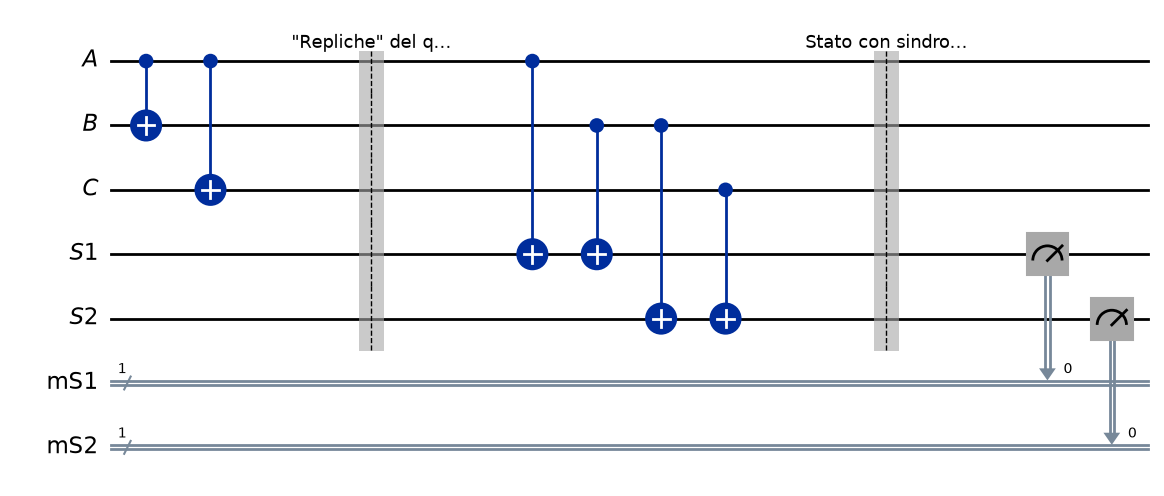
\includegraphics[width=.9\textwidth]{fig/Chapter-4/quantum.ecc-scheme.png}
\caption{Informazione codificata su più qubit}\label{img:error-correction-codes}
\end{figure}

Per fare due conti, lo stato iniziale è il seguente:
\begin{gather*}
    \ket{psi} = \ket{\phi_A} \otimes \ket{0_B} \otimes \ket{0_C}
\end{gather*}
Andando a considerare che \(\ket{\phi_A} = \alpha \ket{0} + \beta \ket{1}\), si avrà:
\begin{align*}
    \ket{\psi} &= \ket{\phi_A} \otimes \ket{0_B} \otimes \ket{0_C}\\
    &= (\alpha \ket{0} + \beta \ket{1}) \otimes \ket{0_B} \otimes \ket{0_C}\\
    &= \alpha \ket{0_A 0_B 0_C} + \beta \ket{1_A 0_B 0_C}
\end{align*}

Andando ad effettuara le due C-Not, i due termini finali nel secondo elemento dell'equazione passano da 0 ad 1, diventando:
\begin{align*}
    \ket{\psi} &= \alpha \ket{0_A 0_B 0_C} + \beta \ket{1_A 1_B 1_C}
\end{align*}

Ottenendo i qubitlogici. Se si fanno passare per un canale di tipo X-Noise, si avrà che, considerando un solo possibile errore, che gli stati saranno:
\begin{align*}
    \ket{\psi} &= \alpha \ket{100} + \beta \ket{011}\\
    \ket{\psi} &= \alpha \ket{010} + \beta \ket{101}\\
    \ket{\psi} &= \alpha \ket{001} + \beta \ket{110}
\end{align*}

Definiti tali casi di errore, si va a considerare che, effettuando le interazioni con le ancille, si avrà che:
\begin{itemize}
    \item \(\ket{0_{S1} 0_{S2}}\): Non c'è alcun tipo di errore
    \item \(\ket{0_{S1} 1_{S2}}\): Vi è un errore sul terzo qubit (di tipo X-Noise)
    \item \(\ket{1_{S1} 0_{S2}}\): Vi è un errore sul primo qubit
    \item \(\ket{1_{S1} 1_{S2}}\): Vi è un errore sul secondo qubit
\end{itemize}

La misura mediante le ancille permette di non perturbare in alcun modo lo stato cercando di estrarre informazioni solo su eventuali cambiamenti avvenuti ai qubit. Questo seguendo la seconda parte dello schema visualizzabile alla figura [\ref{img:error-correction-codes}]. Da tale schema è possibile immaginare anche un eventuale controllo che va a pilotare una porta X controllata da bit classici. Effettuata la detection dell'errore questo viene corretto prima della detection. Lo schema del decodificatore si visualizza all'immagine [\ref{img:quantum-decoder}].

\begin{figure}[H]
\centering
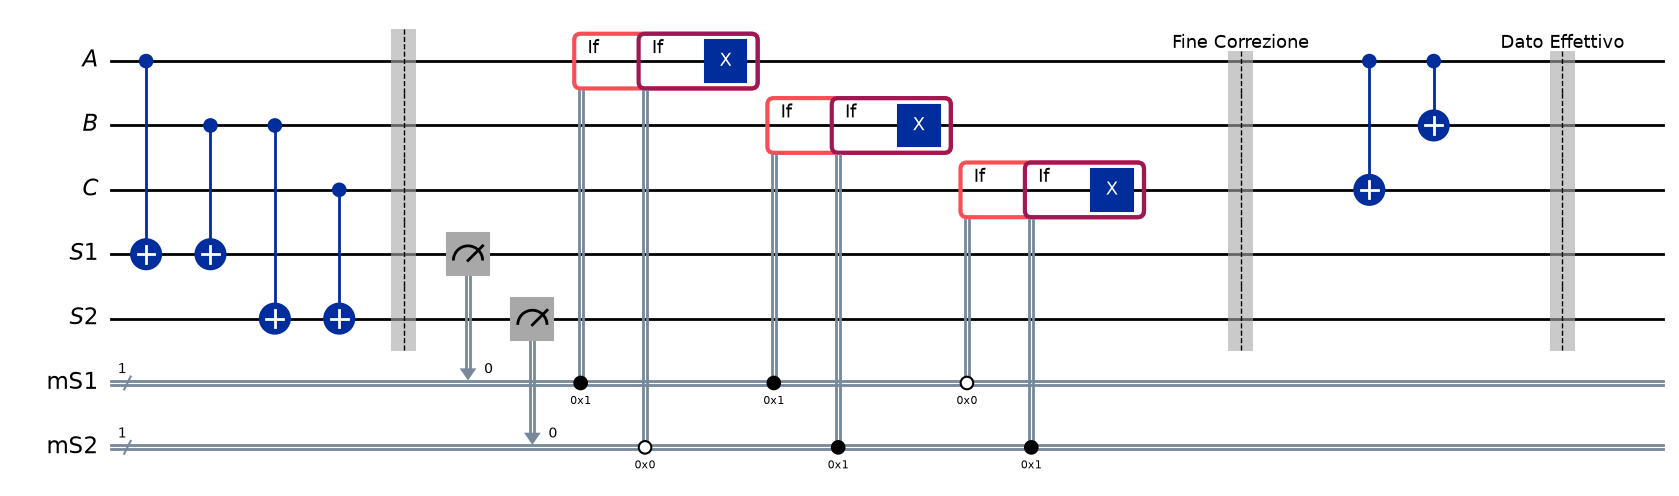
\includegraphics[width=\textwidth]{fig/Chapter-4/decoding.png}
\caption{Quantum Error Correction and Decoding}\label{img:quantum-decoder}
\end{figure}

Alla fine del circuito [\ref{img:quantum-decoder}] il primo qubit sarà esattamente il qubit che si è voluto inviare, questo a meno di al più un errore di bit flip sul dato inviato. Nonostante stiamo parlando di comunicazioni tali sistemi si vanno ad utilizzare anche su delle strutture fisiche locali. Un esempio di applicazione di tali sistemi sono i surface-code, che vanno ad utilizzare in maniera morbosa tale sistema.






\printbibliography[heading=bibintoc, title={Bibliografia}]


\end{document}